\documentclass[acmtocl]{acmtrans2m}

\usepackage{graphicx}

\newtheorem{theorem}{Theorem}[section]
\newtheorem{conjecture}[theorem]{Conjecture}
\newtheorem{corollary}[theorem]{Corollary}
\newtheorem{proposition}[theorem]{Proposition}
\newtheorem{lemma}[theorem]{Lemma}
\newdef{definition}[theorem]{Definition}
\newdef{remark}[theorem]{Remark}

\newcommand{\comment}[1]{}

\title{An Experimental Study of Sorting and Branch Prediction}

\author{
PAUL BIGGAR\footnote[1]{Supported by the Irish Research Council for Science,
Engineering and Technology (IRCSET).}, NICHOLAS NASH\footnotemark[1], KEVIN
WILLIAMS\footnote[2]{Supported by the Irish Research Council for Science,
Engineering and Technology (IRCSET) and IBM.}, and DAVID GREGG \\University of
Dublin, Trinity College
}

\begin{abstract} 
Sorting is one of the most important and well studied problems
in Computer Science. Many good algorithms are known which offer various
trade-offs in efficiency, simplicity, memory use, and other factors. However,
these algorithms do not take into account features of modern computer
architectures that significantly influence performance. Caches and branch
predictors are two such features, and while there has been a significant amount
of research into the cache performance of general purpose sorting algorithms,
there has been little research on their branch prediction properties. In this
paper we empirically examine the behaviour of the branches in all the most
common sorting algorithms. We also consider the interaction of cache
optimization on the predictability of the branches in these algorithms.  We find
insertion sort to have the fewest branch mispredictions of any comparison-based
sorting algorithm, that bubble and shaker sort operate in a fashion which makes
their branches highly unpredictable, that the unpredictability of shellsort's
branches improves its caching behaviour and that several cache optimizations
have little effect on mergesort's branch mispredictions. We find also that
optimizations to quicksort -- for example the choice of pivot -- have a strong
influence on the predictability of its branches. We point out a simple way of
removing branch instructions from a classic heapsort implementation, and show
also that unrolling a loop in a cache optimized heapsort implementation improves
the predicitability of its branches. Finally, we note that when sorting random
data two-level adaptive branch predictors are usually no better than simpler
bimodal predictors. This is despite the fact that two-level adaptive predictors
are almost always superior to bimodal predictors in general.
\end{abstract}

\category{E.5}{Data}{Files}[Sorting/Searching]
\category{C.1.1}{Computer Systems Organization}{Processor Architectures, Other
Architecture Styles}[Pipeline processors]
\terms{Algorithms, Experimentation, Measurement, Performance}
\keywords{Sorting, Branch Prediction, Pipeline Architectures, Caching}

\begin{document}

\begin{bottomstuff}
Corresponding author's address: David Gregg, Department of Computer
Science, University of Dublin, Trinity College, Dublin 2, Ireland. {\tt
David.Gregg@cs.tcd.ie}.
\end{bottomstuff}

\maketitle

\section{Motivation}
Classical analyses of algorithms make simplifying assumptions about the cost of
different machine instructions. For example, the RAM model used for establishing
asymptotic bounds and Knuth's MIX machine code both make drastically simplifying
assumptions about the cost of machine instructions \cite{KnuthVol1_97}. More
recently researchers have recognized that on modern computers the cost of
accessing memory can vary dramatically depending on whether the data can be
found in the first-level cache, or must be fetched from a lower level of cache
or even main memory.  This has spawned a great deal of research on
cache-efficient searching and sorting
\cite{Nyberg+94,Agarwal96,LaMarca96b,LaMarca96a,LaMarca97,Xiao+00,Rahman+01,Wickremesinghe+02}.

Another type of instruction whose cost can vary dramatically is the conditional
branch. Modern pipelined processors depend on \emph{branch prediction} for much
of their performance.  If the direction of a conditional branch is correctly
predicted ahead of time, the cost of the conditional branch may be as little as
the cost of, say, an integer add instruction. If, on the other hand, the branch
is mispredicted the processor must flush its pipeline, and restart from the
correct target of the branch. This cost is typically a large multiple of the
cost of executing a correctly-predicted branch. For example, Intel Pentium 4
processors \cite{Intel248966-010,Intel249438-01} have pipelines of up to 31
stages, meaning that a branch misprediction will cost around 30 cycles.
Fortunately, the branches in most programs are very predictable, so branch
mispredictions are usually rare. Indeed, prediction accuracies of greater than
90\% are typical \cite{Uht+97} with the best predictors.

The cost of executing branches is particularly important for sorting because the
inner-loops of most sorting algorithms consist of comparisons of items to be
sorted. Thus, the predictability of these comparison branches is critical to the
performance of sorting algorithms. In this paper we study the predictability of
branches in most of the major sorting algorithms.  We focus on the behaviour of
the branches whose outcome depends on a comparison of keys presented to the
sorting algorithm in its input. Throughout this paper we refer to such branches
as \textit{comparison branches}. Branches associated with controlling simpler
aspects of the control flow of the algorithms are of much less interest because
they are generally almost perfectly predictable.  We also examine cache
conscious variations of many of the algorithms, and show how optimizations for
the cache influence the level of branch mispredictions.

\section{Branch prediction}
\label{branch_prediction}

Branches are a type of instruction used for defining the flow control of
programs. In high level languages they result from the use of statements like
\texttt{if}, \texttt{while} and their variants. Branches can be either
\textit{taken}, indicating that the address they provide is the new value for
the program counter, or they can be \textit{not-taken}, in which case sequential
execution continues as though the branch had not been present.

Branch instructions pose a difficulty for pipelined processors. In a pipelined
processor, while the program counter points to a particular instruction, a
potentially large number of subsequent instructions are in a partially completed
state.  Until it is known whether a branch is taken or not-taken, it is not
possible to know what the next instructions to be executed are.  If the
processor cannot tell what these next instructions are, it cannot fill its
pipeline.  To keep the utilization of the pipeline at a reasonable level, modern
processors attempt to anticipate the outcome of branch instructions by employing
\textit{branch predictors}. A good discussion of pipelining and its associated
issues can be found in Hennessy and Patterson \citeyear{HennessyPatterson90}.
 
There are several kinds of branch predictors: static, semi-static and dynamic.
We use only dynamic predictors in our experiments, because they are most
commonly used in real processors. The statistics in the following paragraphs are
taken from those derived by Uht \textit{et al} \citeyear{Uht+97}, over the
SPECint92 benchmarking suite. 

The simplest type of dynamic predictor is referred to as a \textit{1-bit}
predictor. It keeps a table recording, at each entry, whether a particular
branch was taken or not-taken.  Using the table, it predicts that a branch will
go the same way as it went on its previous execution. 1-bit predictors achieve
77\% to 79\% accuracy.

We refer to a 2-bit dynamic predictor as a \textit{bimodal} predictor. A bimodal
predictor operates in the same manner as a 1-bit predictor but each table entry
can be thought of  as maintaining a counter from 0 to 3. The counter decrements
on each taken branch (with the exception of when the count is 0), and increments
on each not-taken branch (with the exception of when the count is 3). With
counts equal to 0 or 1 the next branch is predicted as taken, with counts of 2
or 3 the branch is predicted not-taken.  When the counter is 0, we say the
predictor is in the \textit{strongly taken} state, since the branch must be
not-taken twice before the not-taken direction will be predicted again. When the
counter is 1 we say the predictor is in the \textit{taken} state. Similarly
counts of 2 and 3 are referred to as \textit{not-taken} and \textit{strongly
not-taken} respectively. Bimodal predictors achieve 78\% to 89\% accuracy.

Finally, some branch predictors attempt to exploit correlations in branch
outcomes to improve accuracy. A \textit{two-level adaptive} predictor maintains
a \textit{branch history register}. This register records the outcomes of a
number of previous branch instructions. For example, a register contents of
\texttt{110010} indicates that the 6 previous branch outcomes were taken, taken,
not-taken, not-taken, taken and not-taken.  For each branch, this register is
used to index a table of bimodal predictors.  The program counter can also be
included in the index, either concatenated or XORed with the indexing register.
Two-level adpative predictors are accurate about 93\% of the time.

In all the above, due to the size of the predictor table branches can collide.
That is, two different branches can map to the same table location, often
reducing accuracy.

\section{Experimental Setup}
 
We used truly random data provided by Haahr \citeyear{Random} in all our
experiments. We used ten chunks of random data containing $2^{22}$ (4194304)
keys.  Where a particular experiment used only part of the keys in a chunk, it
used the left-most keys.  Our results are averaged over these chunks of data.

In order to experiment with a variety of cache and branch prediction results we
used the SimpleScalar PISA processor simulator version 3
\cite{SimpleScalarTutorialv4}.  We used \texttt{sim-cache} and
\texttt{sim-bpred} to generate results for caching and branch prediction
characteristics respectively.

We used a variety of cache configurations; generally speaking we used an 8 KB
level 1 data cache, 8 KB level 1 instruction cache, and a shared 2 MB
instruction and data level 2 cache, all with 32 byte cache lines.  We also
experimented with both direct mapped and fully associative caches. When
presenting results where the cache configuration is important, we will describe
the precise configuration used. We present results here only for direct mapped
caches. The results for fully associative caches are similar, as we show in our
technical report \cite{BiggarGregg05}, which contains complete results for a
large number of branch predictor and cache configurations. 

For the measurements taken using SimpleScalar, we used power of two sized sets
of random keys ranging from $2^{12}$ to $2^{22}$ keys in size.  This is with the
exception of the quadratic time sorting algorithms, for which the maximum set
size used was $2^{16}$ keys. This was done because of the very significant time
it takes such algorithms to sort large inputs.

It takes time to fill arrays, and this can distort the relationship between the
results for small set sizes, and larger set sizes, for which this time is
amortised. As a result, we measured this time, and subtracted it from our
results.  However, this practice also distorts the results. It removes
compulsory cache misses from the results, so long as the data fits in the cache.
When the data does not fit in the cache, the keys from the start of the array
are faulted, with the effect that capacity misses reoccur, which are not
discounted. 

For branch prediction we simulated both bimodal and two-level adaptive
predictors.  We used power of two sized tables for the branch predictors.  We
used tables containing between $2^{11}$ and $2^{14}$ predictors.  When
presenting branch prediction results, the predictor configurations will be
described precisely.  SimpleScalar's \texttt{sim-bpred} provides total results
over all the branches in a program. It is often desirable to examine particular
branches individually however.  In order to do so, we added our own simulations
of branch predictors to the programs. For our own simulations we average the
results of each branch over ten runs of random data containing $2^{22}$ keys.

Finally we used \textit{PapiEx} \cite{PapiExManual} to access performance
counters on a Pentium 4 1.6 Ghz. This allows cycle counts (i.e. running times)
to be determined for the sorting algorithms on a real processor.  The results
presented from these tests are averaged over 1024 runs and use the system's
random number generator to provide data. The data ranged in size from $2^{12}$
to $2^{22}$ keys in size.  The processor we used had an 8-way associative 256KB
level 2 cache with 64-byte cache lines. The separate data and instruction level
1 caches are 4-way associative, 8KB in size and have 32-byte cache lines.  The
Pentium 4 uses an unspecified form of dynamic branch prediction. A reference
manual \cite{Intel248966-010} mentions a branch history register, so it is
probable that the scheme is similar to two-level adaptive.


\section{Elementary sorts}

We begin by analysing the branch prediction behaviour of a number of common
elementary sorting algorithms, each operating in $O(n^2)$ time. The main
practical advantage of these algorithms is their simplicity, which generally
allows them to operate faster than algorithms with $O(n \lg n)$ time complexity
for small inputs. Indeed, as we will see later, optimized versions of 
$O(n \lg n)$ sorts use calls to elementary sorts for small inputs.  Knuth
\citeyear{KnuthVol3_98} provides a good exposition of these elementary sorting
algorithms (as well as basic versions of the sorting algorithms we shall examine
in later sections).

\subsection{Selection Sort}
\label{selection_sort}

Selection sort is a very simple quadratic time sorting algorithm which begins by
sequentially searching for the smallest key in its input and moving it into
position. The algorithm continues by repeatedly searching for and then moving
the smallest key in the unsorted section of its input into the appropriate
position. The inner-loop of selection sort, which is run a total of $n - 1$
times on an input \texttt{a[0..n - 1]} is shown below

\begin{verbatim}
  min = i;
  for(j = i + 1; j < n; j++)
    if(a[j] < a[min]) min = j;
  swap(a[i], a[min]);
\end{verbatim}

It is easy to see that selection sort performs approximately $n^2/2$ comparisons
and exactly $n - 1$ exchanges.  On the $j^{th}$ iteration of the inner-loop the
comparison branch is taken if \texttt{a[j]} is the minimum of \texttt{a[i..j]},
which occurs with probability $1 / (j - i + 1)$\footnote{Throughout this paper,
for the purpose of analysis we make the usual assumption that the input to be
sorted consists of a random permutation of $\lbrace1, .., n\rbrace$.}.  The
expected number of times the branch is taken on the first iteration is thus
given by $H_n - 1$ where $H_n = \sum_{i = 1}^n 1/i$ is the $n^{th}$ harmonic
number \cite{KnuthVol1_97}.  Since $H_n \approx \ln n$, and 
$\sum_{i = 1}^n H_i = O(n \ln n)$ the comparison branch will be highly
predictable. As expected, Figure \ref{elementary_sorts}(a) shows that number of
mispredictions per key grows in a similar fashion to $\ln n$.

If the array is initially in sorted order, then the value of \texttt{min} will
never change in the inner-loop. Since this implies the comparison branch is
never taken, it will be almost perfectly predictable. Similarly, if the array is
sorted in reverse order, the value of \texttt{min} must change at every element.
That is, the comparison branch is taken at every element, and the branch is
therefore almost perfectly predictable.  From the point of view of branch
prediction, frequent changes (preferably with no simple pattern) are the main
indicator of poor performance, rather than the absolute number of times that the
branch resolves in each direction. The worst case for selection sort would be an
array which is partially sorted in reverse order; the value of \texttt{min}
would change frequently, but not predictably so.  Figure
\ref{elementary_sorts}(a) shows the behaviour of selection sort's branches.

\subsection{Insertion Sort}
\label{insertion_sort}

Insertion sort is another simple algorithm with quadratic worst case time. It
works by iterating the inner-loop below a total of $n - 1$ times over its input

\begin{verbatim}
   item = a[i];
   while(item < a[i - 1]) 
   {
     a[i] = a[i - 1];
     i--;
   }
   a[i] = item;
\end{verbatim}

On the $i^{th}$ iteration \texttt{a[0..i - 1]} is sorted, allowing \texttt{a[i]}
to be placed in the correct position as shown in the inner-loop above. On
average, insertion sort performs approximately $n^2/4$ comparisons and $n^2/4$
assignments in its inner-loop. Thus insertion sort performs around half as many
branches as selection sort.

A very pleasing property of insertion sort is that it generally causes just a
single branch misprediction per key, as Figure \ref{elementary_sorts}(a) shows.
Typically the inner \texttt{while} loop exit causes this misprediction, when the
correct location for the current item has been found.  In fact, a static
predictor would perform just as well as the two predictors shown, since it would
mispredict exactly once per key.

\begin{figure}
\centering
\begin{tabular}{cc}
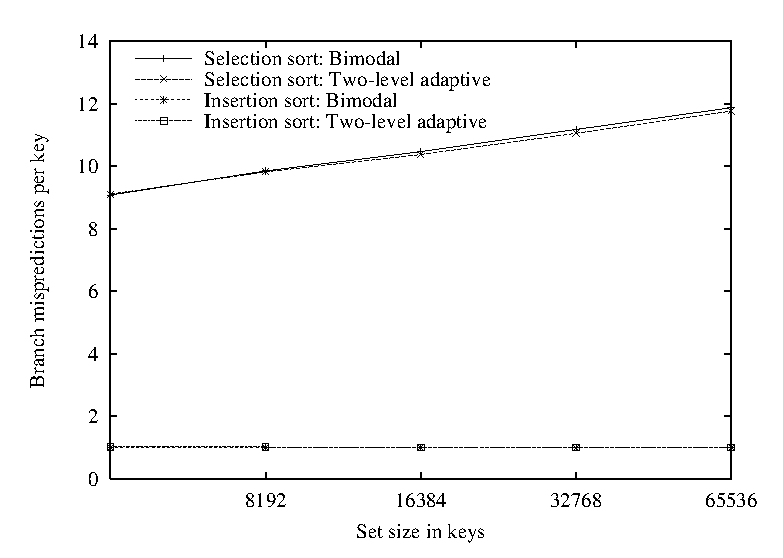
\includegraphics[width=0.48\textwidth]{plots/selection_insertion_sort_branches.eps} & 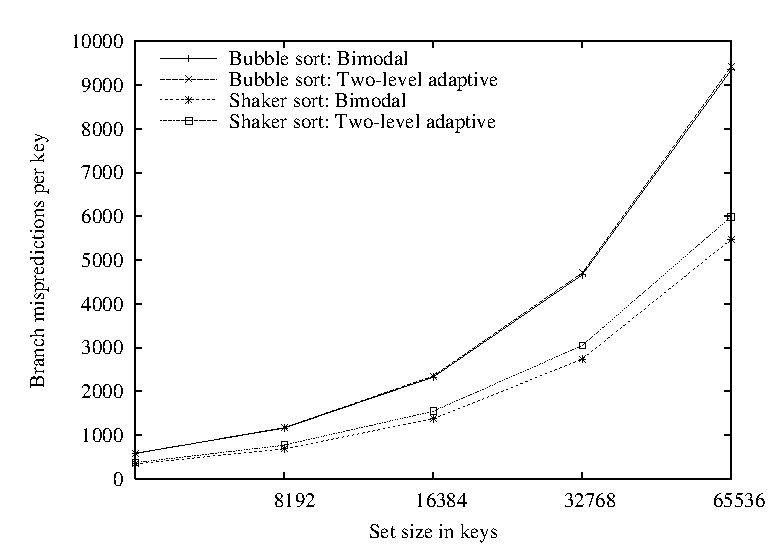
\includegraphics[width=0.48\textwidth]{plots/bubble_shaker_sort_branches.eps} \\
(a) & (b) \\
\end{tabular}
\caption{(a) Shows the branch mispredictions for selection and insertion sort
using bimodal and two-level adaptive predictors both having 4096 table entries.
It is noteworthy the simple bimodal predictor has essentially identical
performance to the two-level adaptive predictors. (b) Shows the branch
mispredictions for bubble and shaker sort using bimodal and two-level adaptive
predictors, again both having 4096 table entries. For bubble sort the bimodal
and two-level adaptive predictors have close to identical performance. However,
for shaker sort the simple bimodal predictor results in fewer mispredictions
than the two-level adaptive predictor. We also note that as a result of the
partial sorting performed by bubble and shaker sort they incur far more branch
mispredictions per key than other $O(n^2)$ sorting algorithms.
\texttt{sim-bpred} was used to simulate the branch predictors in both (a) and
(b). The two-level adaptive predictors used 10-bit history registers.}
\label{elementary_sorts}
\end{figure}


\subsection{Bubble sort}
\label{bubble_sort}

Bubble sort is another simple sorting algorithm, although notoriously
inefficient. It works by iterating the loop shown below at most $n - 1$ times on
an input \texttt{a[0..n - 1]}.

\begin{verbatim}
for(j = 0; j < n - i - 1; j++)
{
    if(a[j + 1] < a[j])
       swap(a[j + 1], a[j]);
}

\end{verbatim} 

In this code $i$ is the outer-loop iteration counter, and begins at 0 and counts
towards $n - 1$. Bubble sort uses information yielded by the comparisons which
selection sort simply discards. After a full iteration of the inner-loop shown
larger elements have moved to the right, closer to their final location.

Shaker sort is a variation of bubble sort in which there are two inner-loops
which are alternated. One is the inner-loop shown above. The other inner-loop
scans right-to-left moving small elements to the left in the same manner as
moving larger elements to the right has just been described.  Although shaker
sort has the same worst-case time as bubble sort, it is generally more efficient
in practice.

Figure \ref{elementary_sorts}(b) shows the number of branch mispredictions per
key for bubble and shaker sort. As the data set gets large, bubble sort causes
nearly 10000 branch mispredictions per key. Shaker sort executes a lot fewer
branches, and so has fewer mispredictions, but the rate of misprediction is
similar.

To understand the high misprediction rate of bubble sort we define $Q^k_l$ as
the probability that $l^{th}$ inner-loop comparison branch is taken on the
$k^{th}$ outer-loop iteration, $1 \leq k < n$. It turns out that

\begin{equation}
\label{bubble_equation}
Q^k_l = 
\left\{ 
\begin{array}{ll}
  \frac{l}{l + k} & \quad \mbox{if $l \leq n - k$}\\
  0 & \quad \mbox{otherwise}\\ 
\end{array} 
\right. 
\end{equation}

\noindent
This is a result of the fact that the $l^{th}$ comparison branch of the
inner-loop is taken only if \texttt{a[l]} is not larger than all of
\texttt{a[0..l - 1]}.  For this to be the case, the $(l + 1)^{th}$ branch in the
previous outer-loop iteration must have been taken, since otherwise the previous
iteration of the outer-loop left the maximum of \texttt{a[0..l - 1]} in
\texttt{a[l]}.  The probability that the $(l + 1)^{th}$ branch of the
previous outer-loop iteration is taken is $Q^{k - 1}_{l + 1}$. Given that the
$(l + 1)^{th}$ branch of the previous outer-loop iteration was taken, the
probability that \texttt{a[j]} is not larger than all of \texttt{a[0..l - 1]} is
$1 - 1/(l + 1)$, thus,

\[
Q^k_l = Q^{k-1}_{l+1}\left(1 - \frac{1}{l + 1} \right)
\] 

\noindent
The bases $Q^{1}_l = 1 - 1 / (l + 1)$ for $1 \leq l < n$ and $Q^1_n = 0$ give
the solution shown in Equation \ref{bubble_equation}.  It is easy to see that in
the first outer-loop iteration ($k = 1$) the comparison branch is very likely to
be taken, whereas in the last outer-loop iteration ($k = n - 1$), the comparison
branch is very unlikely to be taken. Moving between these two extremes causes
the intermediate branches to be unpredictable. The remainder of this section
examines this phenomenon in more detail.

In order to analyse the behaviour of bubble sort when a bimodal predictor is
used, it is useful to make use of the \textit{steady state predictability}
function. This function generally gives a good estimate of the probability that
a particular branch will be correctly predicted, given that we know the
probability that the branch will be taken. For a bimodal predictor this function
is given by

\begin{equation}
CP(p) = \frac{3p^2 - 3p + 1}{2p^2 - 2p + 1}
\label{CP_equation}
\end{equation}

\noindent Where $p$ is the probability that the branch in question will be
taken. Although the derivation of this function is simple, we relegate it to the
appendix because we wish to focus mainly on our experimental results. $CP$ can
be used to examine the predictability of the branches in bubble sort as the
outer-loop iterates.  Bubble sort executes $n - k$ comparison branches on its
$k^{th}$ outer-loop iteration. Thus, using Equation \ref{bubble_equation} the
average probability that the comparison branch is taken on the $k^{th}$
outer-loop iteration is 

\begin{eqnarray*}
Q^k_{avg} &=& \frac{1}{n - k} \sum_{l = 1}^{n - k} \frac{l}{l + k} \\
          &=& 1 + \frac{k}{n - k}(H_k - H_n)\\
%  &=& \frac{n - k - k(H_n - H_k)}{n - k}\\
         &\approx& 1 + \frac{k}{n - k}\ln\frac{k}{n}
\end{eqnarray*}

\noindent
Where $H_n$ denotes the $n^{th}$ harmonic number. An approximation to the
predictability of the comparison branch of bubble sort on the $k^{th}$ iteration
is then given by $CP(Q^k_{avg})$.  Figure \ref{bubble_predictability}(a) plots
this, showing how the predictability of the comparison branch varies with the
number of outer-loop iterations. Figure \ref{bubble_predictability}(b) shows the
measured number of correctly predicted branches as the outer-loop iterates,
these results correspond approximately with what was obtained analytically in
Figure \ref{bubble_predictability}(a).

\begin{figure}
\centering
\begin{tabular}{cc}
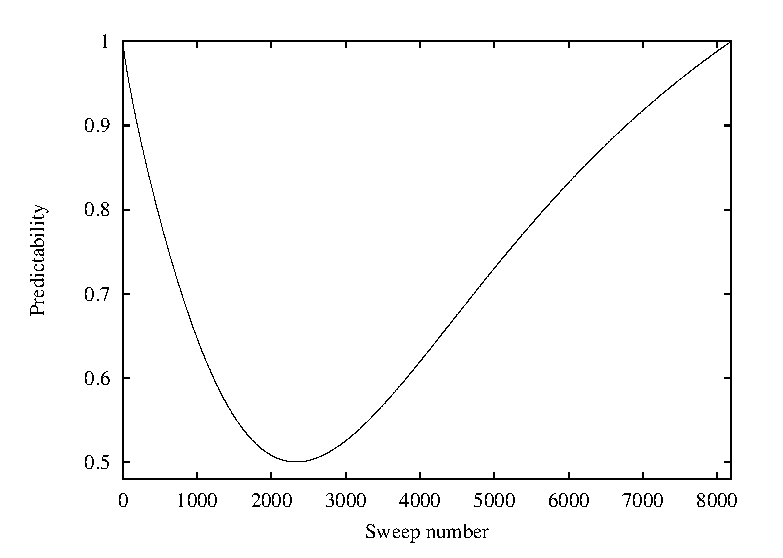
\includegraphics[width=0.48\textwidth]{plots/bubble_predictability.eps} & 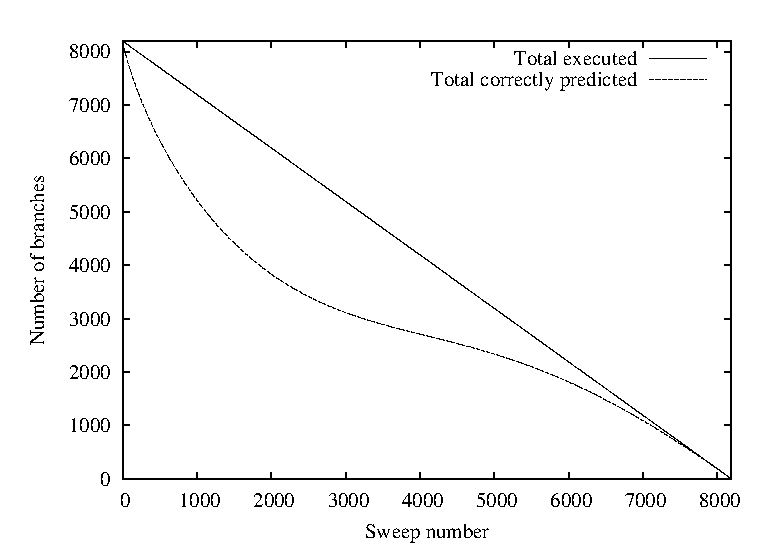
\includegraphics[width=0.48\textwidth]{plots/bubble_sweep_misses.eps} \\
(a) & (b) \\
\end{tabular}
\caption{(a) Shows $CP(Q^k_{avg})$ as the sweep number, $k$, increases (i.e. as
the outer-loop iterates). This gives a good approximation to the predictability
of the comparison branch of bubble sort. (b) Shows the number of correctly
predicted branches in bubble sort, as well as the number of executed branches.
Initially the number of correctly predicted branches is close to the number
executed, however, the number of correctly predicted branches rapidly decreases
as the sweep number increases. Gradually, the branches become predictable again.
These trends correspond to the variation in predictability shown in (a). The
results of (b) were obtained using our own software simulated bimodal predictor
averaged over a large number of arrays with 8192 elements. Note also that in (b)
the version of bubble sort used does not terminate early if no swaps are
performed for an entire execution of the inner-loop.  }
\label{bubble_predictability}
\end{figure}

Initially the branches are quite predictable, however their predictability
reduces quite rapidly as the outer-loop iterates.  The incremental movement of
large keys to the right in bubble sort causes this degredation in the
predictability of its branches. As the data becomes close to being fully sorted
the predictability of the branches improves again. The partial sorting bubble
sort performs allows it to potentially converge to fully sorted data in fewer
outer-loop iterations than selection sort. We can detect that the data is sorted
early if the branch shown in the inner-loop above is never taken for a whole
iteration. However, this partial sorting also greatly increases the number of
branch mispredictions bubble sort incurs, substantially slowing it over
selection sort or insertion sort.

\subsection{Remarks}

Our results clearly demonstrate the importance of branch prediction for the
elementary sorting algorithms.  Our shaker sort implementation has fewer cache
misses than our selection sort implementation, as Figure \ref{shaker_plots}(a)
shows.  It also has a lower instruction count than selection sort. However it is
slower due to branch mispredictions, as Figure \ref{shaker_plots}(b) shows.
Figure \ref{elementary_sorts} shows the contrast between the branch prediction
performance of selection sort and bubble or shaker sort. Where selection sort
causes on average fewer than 12 mispredictions per key for a set size of 65536
keys, bubble and shaker sort cause many thousands.  Insertion sort behaves even
better than selection sort, causing almost a single misprediction per key. Since
insertion sort also has the fewest cache misses it has much to recommend it as
an elementary sorting algorithm. It is bubble sort's partial sorting behaviour
that wreaks havoc with branch prediction, adding further weight to Knuth's
\citeyear{KnuthVol3_98} point of view that it has very little to recommend it,
besides a catchy name and some interesting theoretical problems it poses. 

Finally our results show that over these elementary sorting algorithms two-level
adaptive branch predictors are no better than simpler bimodal predictors.  This
is noteworthy, because two-level predictors are similar to, or sigificantly more
accurate than bimodal predictors for almost all other types of branches
\cite{Uht+97}.  In fact, a bimodal predictor out-performs a two-level adaptive
predictor for shaker sort, as is shown in Figure \ref{elementary_sorts}(b).

\begin{figure}
\centering
\begin{tabular}{cc}
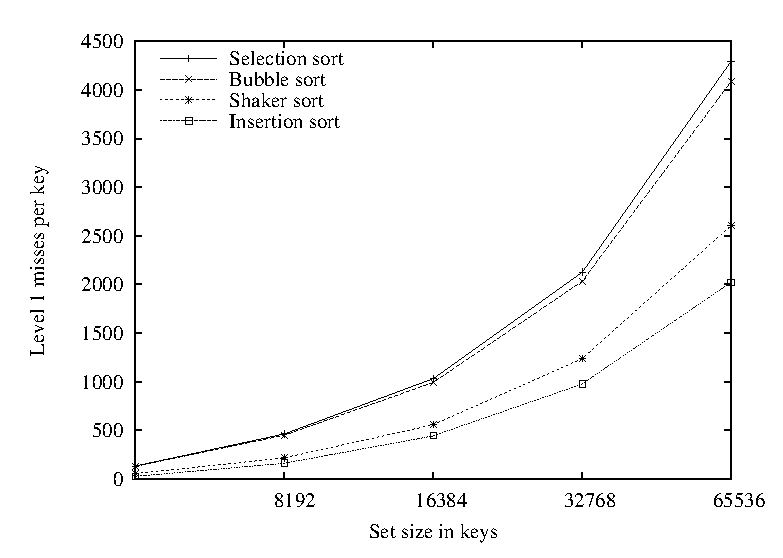
\includegraphics[width=0.48\textwidth]{plots/elementary_cache1_misses.eps} & 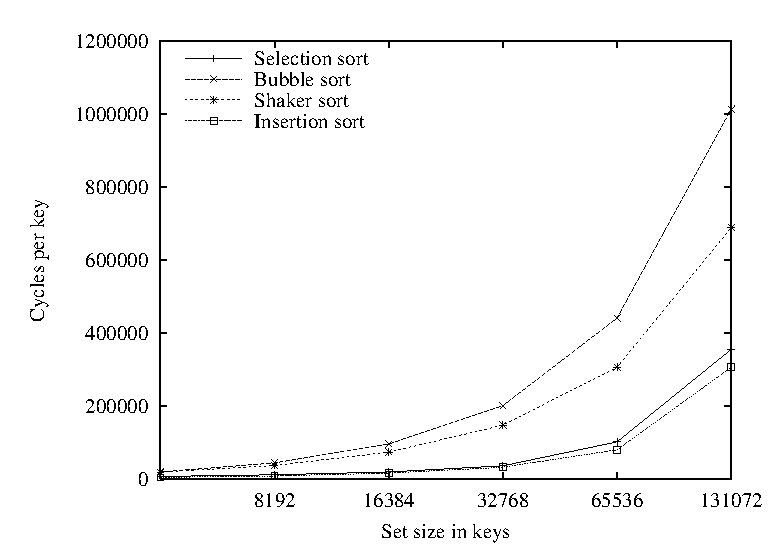
\includegraphics[width=0.48\textwidth]{plots/elementary_cycles.eps}\\
(a) & (b) \\
\end{tabular}
\caption{(a) Shows the level 1 cache misses of the elementary sorting
algorithms.  These results were obtained by using \texttt{sim-cache} to simulate
an 8KB direct mapped level 1 cache with 32 byte cache lines. Note that there are
no level 2 cache misses since the simulated 2nd level cache is 2MB in size.  (b)
Shows the number of cycles per key for the elementary sorting algorithms.
Despite bubble and shaker sort having better cache performance than selection
sort, the vast number of branch mispredictions (see Figure
\ref{elementary_sorts}(b)) they cause make them less efficient than selection
sort in practice.  These results were measured using hardware performance
counters on a Pentium 4.}
\label{shaker_plots}
\end{figure}

\section{Shellsort}

Shellsort \cite{Shell59} was the first in-place sorting algorithm with time
complexity better than $O(n^2)$.  Algorithms like selection and bubble sort use
each comparison to resolve at most one inversion (an inversion is a pair of keys
in the input which appear in the wrong order) in the input, and it is well known
that this restricts their average case running time to be in $O(n^2)$
\cite{KnuthVol3_98}. Shellsort uses each comparison to resolve more than one
inversion, giving better performance.

Shellsort uses a sequence of decreasing integers $h_1, h_2, \ldots, h_k$ with
$h_k = 1$, called increments.  On the $i^{th}$ of its $k$ iterations, shellsort
performs an insertion sort but treats \texttt{a[j]} and \texttt{a[j + $h_i$]} as
though they were adjacent (rather than a normal insertion sort, which treats
\texttt{a[j]} and \texttt{a[j + 1]} as adjacent). 

The choice of increments influences shellsort's asymptotic behaviour.  We used
Gonnet's increments \cite{Gonnet+91} for our implementation, because we found
them to be efficient empirically. Using Gonnet's increments $h_i = \lfloor
\frac{5}{11} h_{i - 1} \rfloor$, with $h_1 = \lfloor \frac{5}{11}n \rfloor$ and
the final increment being 1 as usual.

We use a straightforward implementation of shellsort, except we perform the
final iteration (i.e. the iteration in which we perform a standard insertion
sort because the increment is 1) separately.  For this final insertion sort we
extract $\min(a[0], \ldots, a[9])$ as a sentinel, removing the need for a bounds
check in its inner-loop. This also simplifies the bounds checks on the
outer-most loop of the other iterations.

\subsection{Branch Prediction Results}

The behaviour of the comparison branches in shellsort is simple to analyse.
There are $\lfloor \log_\frac{11}{5} n \rfloor$ passes, with each pass
performing an insertion sort (using the current increment). As we saw in Section
\ref{insertion_sort} insertion sort causes about one branch misprediction per
key, thus we expect about $n \lfloor \log_\frac{11}{5}n \rfloor$ mispredictions
in total, and about $\lfloor \log_\frac{11}{5}n \rfloor$ mispredictions per key. 

Figure \ref{shellsort_results_figs}(a) shows the branch mispredictions per key
on average for our shellsort implementations, with bimodal and two-level
adaptive predictors.  The scale on the x-axis is logarithmic, and the plots are
nearly straight lines, as we would expect if the branch mispredictions per key
are given by $\lfloor \log_\frac{11}{5} n \rfloor$. For example, the final
measurement on the x-axis is for a set size of 4194304 and here we observe from
the plot approximately 18 misses per key on average, and 
$\lfloor \log_\frac{11}{5} 4194304 \rfloor = 19$.

The comparison branch of the insertion sort inner-loop of shellsort are very
unpredictable, unlike the nearly perfectly predictable branches of a standard
insertion sort.  We measured a predictability of about 50\% on average for this
branch using a simulated bimodal predictor.  A static predictor which predicts
all branches as taken would be ideal for predicting the branches of the
insertion sorts performed by shellsort.  We found that on average, using
Gonnet's increments, a key moves 0.9744 places per iteration (note that a move
is of $h$ positions, where $h$ is the current increment). Thus, although the
insertion sort branch will still cause just a single misprediction per key, its
outcome is not nearly as predictable as a standard insertion sort, where keys on
average are moved a larger number of times per inner-loop iteration.

One might expect shellsort's cache performance to be poor, since it repeatedly
accesses distantly separated keys in its input while the increments are large.
Each such access could potentially cause a cache miss. However, the fact that on
average keys move just 0.9744 places per iteration implies that large numbers of
references in distant parts of the input (which could lead to cache misses) are
not generally necessary.  In fact, our shellsort implementation has better cache
performance in both the level 1 and level 2 cache than for our basic heapsort
implementation as Figure \ref{shellsort_results_figs}(b), and Figure
\ref{shellsort_results_figs}(c) shows.  Indeed, our shellsort implementation
performs significantly better than our basic heapsort implementation as Figure
\ref{shellsort_results_figs}(d) shows (see Section \ref{heapsort} for further
details on our heapsort implementations).

\section{Heapsort}
\label{heapsort}

Another well known general purpose sorting algorithm is heapsort
\cite{Williams64}. Heapsort's running time is $O(n \lg n)$.  Heapsort begins by
constructing a \textit{heap}: a binary tree in which every level except possibly
the deepest is entirely filled, with the deepest level filled from the left. In
addition, a heap must also satisfy the \textit{heap property}: A key is
associated with each node that is always at least as large as the keys
associated with all its children nodes. The sequence of keys resulting from a
pre-order traversal of a heap's nodes can be used to represent it unambiguously
in an array. 

\begin{figure}
\centering
\begin{tabular}{cc}
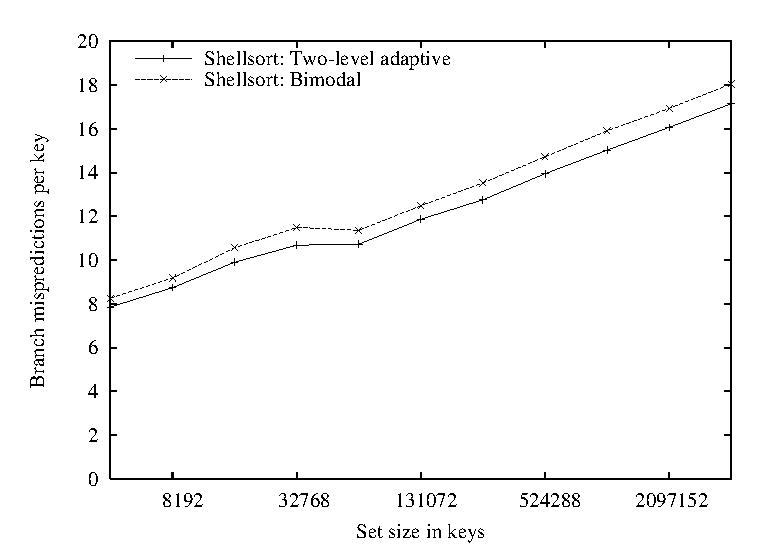
\includegraphics[width=0.48\textwidth]{plots/shellsort_branch_misses.eps} & 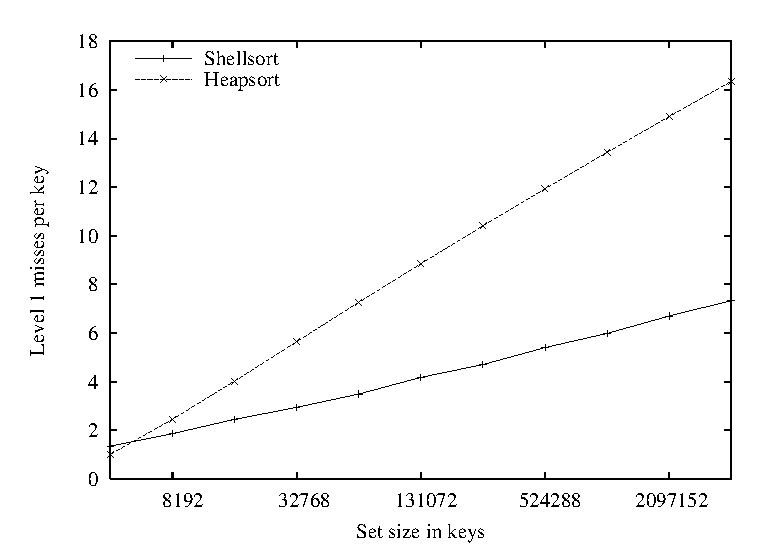
\includegraphics[width=0.48\textwidth]{plots/shell_heap_cache_misses.eps} \\
(a) & (b) \\
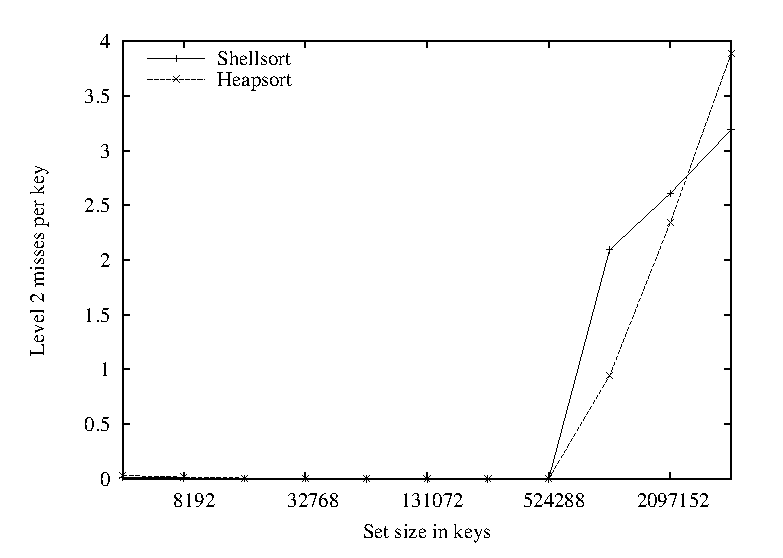
\includegraphics[width=0.48\textwidth]{plots/shell_heap_L2_misses.eps} & 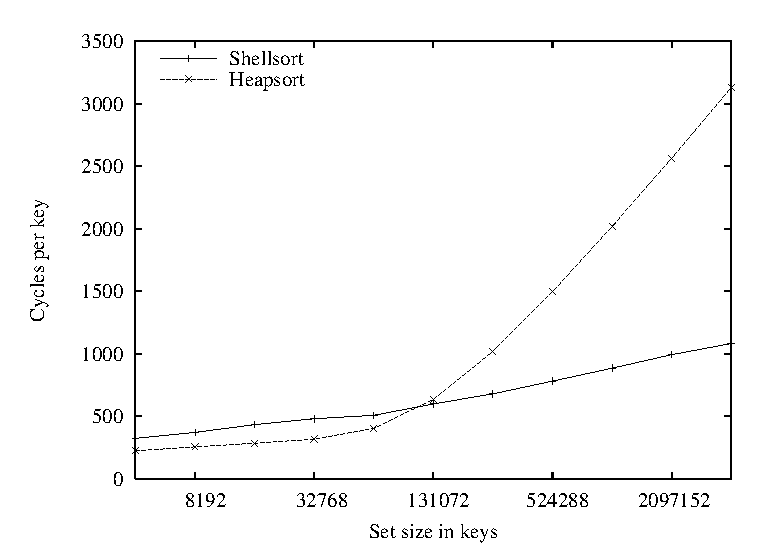
\includegraphics[width=0.48\textwidth]{plots/shell_heap_cycles.eps} \\
(a) & (b) \\
\end{tabular}
\caption{(a) Shows the average branches misses per key for shellsort using a
bimodal and two-level adaptive predictor, both having 4096 table entries.  On
this occasion, the two-level adaptive predictor out-performs the simpler bimodal
predictor. \texttt{sim-bpred} was used to simulate these branch predictors.  (b)
and (c) show that our basic heapsort implementation has inferior cache
performance at both levels of the cache compared to our shellsort
implementation. Shellsort incurs only a small number of cache misses because on
average a key moves just 0.9744 places per iteration. These results use
\texttt{sim-cache} to simulate an 8KB direct mapped level 1 cache and a 2MB
direct mapped level 2 cache both with 32 byte cache lines. Finally (d) shows
that our shellsort implementation out-performs our heapsort implementation,
these results were measured using Pentium 4 hardware performance counters.}
\label{shellsort_results_figs}
\end{figure}


An unordered array can be transformed into a heap in $O(n)$ time, using the
approach of Floyd \citeyear{Floyd64}.  Given a node whose children are heaps but
who may itself violate the heap property, an iteration of Floyd's approach swaps
the node with the larger of its children, and then repeats the same procedure
with the subtree rooted at that child, until the heap property is satisfied or a
leaf is reached. We refer to this as ``sifting down'' a node.  To build the
entire heap, we first sift-down the deepest nodes having children, followed by
their parents, and so on until we reach the root.

Once the heap is built, we gradually destroy it in order to sort. We iterate the
code below $n - 1$ times. 

\begin{verbatim}
    tmp = a[0];
    a[0] = a[--n];
    a[n] = tmp;    
    sift_down(a, 0, n);
\end{verbatim}

\noindent On the $i^{th}$ iteration we swap the largest key, \texttt{a[0]}, with
\texttt{a[n - i]}.  After each swap, the heap property is restored by sifting
down the new root of the heap (an operation with worst case time $O(\lg n)$).
After iteration $i$ the heap contains $n - i$ keys, and is found in
\texttt{a[0..n - i - 1]}. Meanwhile \texttt{a[n - i..n - 1]} contains the $i$
largest keys of the input from smallest to largest.

\subsection{Heapsort Variations}

For our base heapsort implementation, we used the approach described in the
previous section, but removed a bounds check from the sift down procedure by
introducing a sentinel at the cost of no extra instructions. The following
optimization reduced the instruction count by about 10\% on average compared to
an implementation of sift-down which uses a bounds check. We have not seen it
described elsewhere. In a heap, exactly one node has a single left child, all
other nodes have either two children or zero children. On every sift-down, we
compare each node which has children with each of its children. As a result of
the node with a single child, on every sift-down we must check that the node
being compared to its children has a right child as well as a left child. To
avoid this check while building the heap, we can just insert a maximal extra
node at the end of the heap. When destroying the heap however, every second
iteration requires the insertion of this extra node. To avoid this the code for
destroying the heap shown in the previous section is changed to

\begin{verbatim}
    tmp = a[0];
    a[0] = a[--n];
    sift_down(a, 0, n);
    a[n] = tmp;
\end{verbatim}

\noindent 
By not modifying \texttt{a[n - 1]} until after sifting down, it acts as a
sentinel for sift-down. This removes the need for the bounds check without
introducing any extra instructions.

Aside from this optimization, we also applied caching optimizations of LaMarca
and Ladner \citeyear{LaMarca96b} to give several cache-optimized versions of the
algorithm. Firstly, the heap can be padded so that siblings always reside in the
same cache line. Another cache optimization is realised by abandoning Floyd's
heap building method and simply repeatedly growing the heap one array element at
a time, sifting each new key upwards as needed. This greatly improves the
temporal locality of the algorithm when the data does not fit entirely within
the cache. 

To increase the utilization of cache lines (and hence require fewer cache lines
to be fetched) we can use a $k$-ary heap instead of the binary heap that has
been assumed until now. When using a $k$-ary heap, every node having children
(except perhaps one) has $k$ children. When sifting up or down a $k$-ary heap,
the maximum (or minimum, depending on the heap property being used) child must
be found, which requires $k - 1$ comparisons. Of course, as $k$ grows the sort
degenerates to a selection sort. Note also that for a $k$-ary heap, the
optimization described above, which avoids bounds checking while sifting down
cannot be applied. However, it is still more efficient to add a sentinel on
every second iteration of the heap destruction (since this introduces $O(n)$
operations whereas the bounds check in the inner-loop introduces $O(n \lg n)$
operations). For modest values of $k$ a performance improvement can be expected
over a simple binary heap \cite{LaMarca96b}. We experimented with 4-heaps and
8-heaps, combined with the aforementioned cache optimizations.

\subsection{Branch Prediction Results}
\label{heapsort_branch_results_text}

Figure \ref{heapsort_results}(a) shows the average number of branches per key
for our heapsort implementations. We note that the cache-optimized heapsort
implementations execute fewer branches per key than our base heapsort
implementation. Although these algorithms execute fewer branches per key on
average, they cause a larger total number of branch mispredictions than our base
heapsort implementation. Indeed, Figure \ref{heapsort_results}(b) shows that the
base heapsort implementation incurs the fewest branch mispredictions of any of
the algorithms.  This is despite the fact that it is executing more branches on
average.  Figure \ref{heapsort_results}(b) also shows that the simpler bimodal
predictors are generally no worse at predicting branches than the two-level
adaptive predictors. With the exception of shellsort, this is in keeping with
the trend we observed for the other sorting algorithms examined so far.

Notwithstanding the base heapsort implementation having the lowest misprediction
rate, Figure \ref{heapsort_results}(c) shows that the most efficient
implementation on our hardware configuration to be the 8-heap variation of
heapsort, followed by the 4-heap variation.  This suggests the improved cache
performance of these algorithms outweighs their increased level of branch
mispredictions shown in Figure \ref{heapsort_results}(b).

When using a $k$-ary heap, finding the maximum (or minimum) child at a
particular node causes the $i^{th}$ comparison branch to be taken with
probability $1/(1 + i)$. The comparisons behave just like those in selection
sort (see Section \ref{selection_sort}), and are therefore quite predictable.
For our 8-heap we unrolled the loop to find the minimum child into 7 separate
branches.  Figure \ref{heapsort_results}(d) shows the behaviour of these 7
branches, for an unrolled loop.  As expected, the later branches are gradually
taken less often on average, with a corresponding increase in their
predictability.  Unrolling this loop not only removes the loop over-head, but is
also experimentally observed to improve the average prediction accuracy by about
2\% \cite{BiggarGregg05}.  The average steady state predicitability in the
unrolled case, is given by

\[
\frac{1}{7}\sum^7_{i=1}CP\left(\frac{1}{1 + i}\right) \approx 0.724
\]

\noindent Where $CP$ is the steady state predictability function introduced in
Section \ref{bubble_sort}.  Without unrolling, the comparison branch is taken on
average with probability $\frac{1}{7}\sum^7_{i=1}\frac{1}{i + 1}$, and its
predictability can be estimated as

\[
CP\left(\frac{1}{7}\sum^7_{i=1}\frac{1}{1 + i} \right) \approx 0.706
\]

\noindent As is observed experimentally, the unrolled loop results in about a
2\% greater prediction accuracy.

\begin{figure}
\centering
\begin{tabular}{cc}
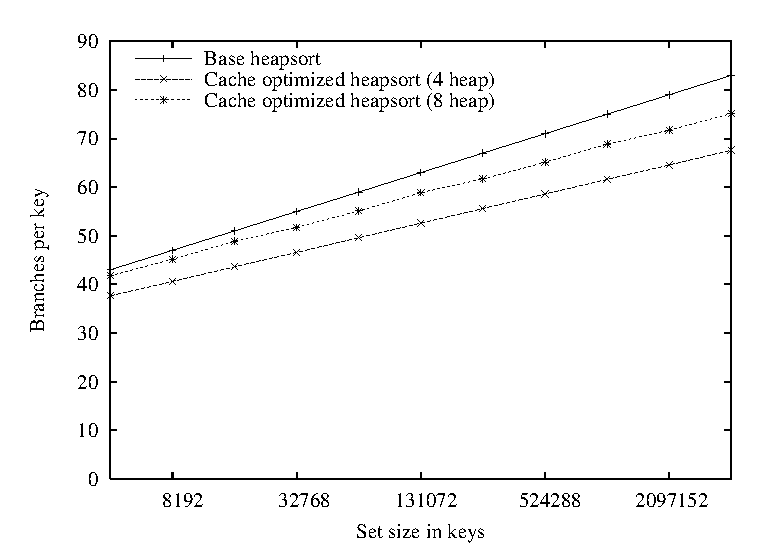
\includegraphics[width=0.48\textwidth]{plots/heapsort_branch_counts.eps} & 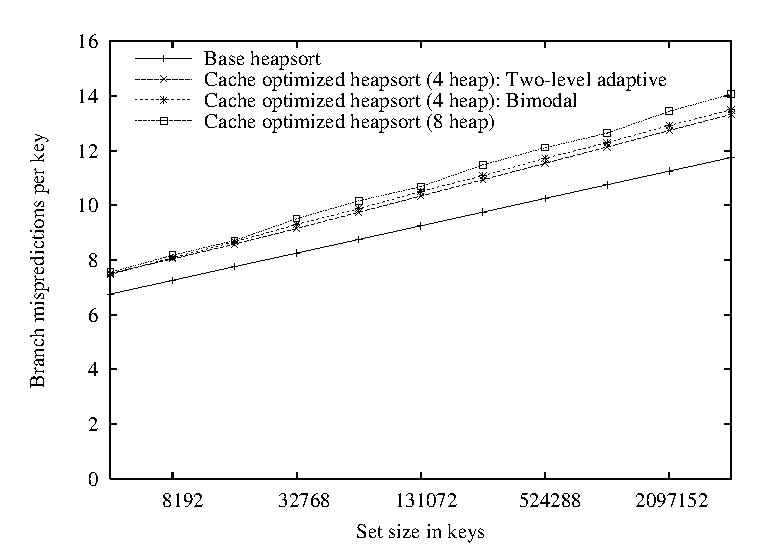
\includegraphics[width=0.48\textwidth]{plots/heapsort_branch_misses.eps}\\
(a) & (b) \\
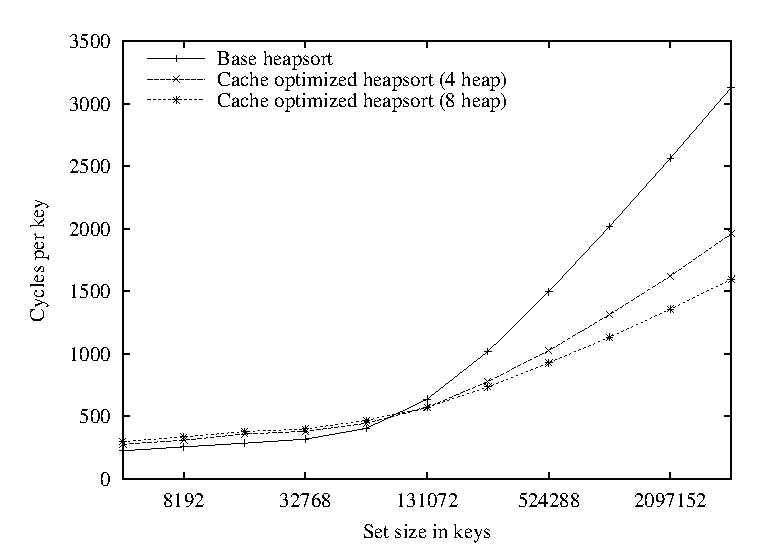
\includegraphics[width=0.48\textwidth]{plots/heapsort_cycle_counts.eps} & 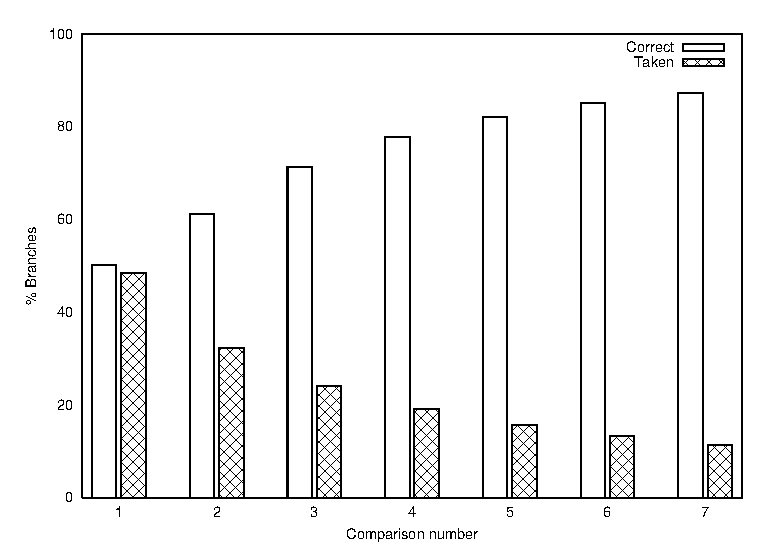
\includegraphics[width=0.48\textwidth]{plots/heapsort_8heap_branches.eps} \\
(c) & (d) \\
\end{tabular}
\caption{Branch prediction and performance characteristics of our heapsort
implementations. (a) Shows the average number of branches per key measured using
\texttt{sim-bpred}. (b) Shows the average branch mispredictions per key for
tables of 4096 predictors, again measured using \texttt{sim-bpred}. The
two-level adaptive (which used a 10-bit history register) and bimodal predictors
have close to identical performance, and to avoid cluttering the diagram only
one instance of a two-level adaptive predictor is shown, the remainder of the
predictors are bimodal. (c) Shows the cycle counts of the algorithms measured
using Pentium 4 hardware performance counters. Note that the Pentium 4 has 32
byte cache lines in its first level cache, and 64 byte cache lines in its second
level cache.  Finally (d) shows the predictability of the unrolled branches
associated with an 8-heap, measured with our own software simulated bimodal
predictor.}
\label{heapsort_results}
\end{figure}

\section{Mergesort}
\label{mergesort}

Mergesort \cite{KnuthVol3_98} is a another $O(n \lg n)$ sorting algorithm, which
works by repeatedly merging pairs of sorted lists into a single sorted list of
twice the length. These merges can be done very simply in linear time and space.
Mergesort's input can be thought of as $n$ sorted lists of length one. To
simplify the description, we assume the number of keys, $n$, is a power of two.
Mergesort makes $\lg n$ passes over the input where the $i^{th}$ pass merges
sorted lists of length $2^{i - 1}$ into sorted lists of length $2^i$. 

\subsection{Mergesort Variations}
\label{mergesort_variations}

For our base mergesort implementation we apply several optimizations.  Firstly,
our mergesort alternates the merge operation between two arrays to avoid
unnecessary copying.  Secondly, a bitonic sort as described by Sedgewick
\citeyear{Sedgewick02}, removes instructions from the inner-loop. A bitonic sort
sorts every second list in reverse, merging then works from the two ends of the
array containing the elements to be merged, terminating when the indices cross.
Since the indices cannot go outside the bounds of the array unless they cross
first, this eliminates the need for a bounds check in the inner-loop.  An
insertion sort is also initially used to create sorted lists of length four,
rather than allowing mergesort to sort these lists.

We also analysed the branch prediction behaviour in several cache conscious
mergesort variations using the work of LaMarca and Ladner \citeyear{LaMarca97}
as a reference, the details of our implementations differ slightly however
\cite{BiggarGregg05}.  Mergesort is not in-place\footnote{Worst case linear time
in-place merging is possible but is generally inefficient in practice, see for
example Katajainen \textit{et al} \citeyear{Katajainen+96}.} and uses an
auxiliary array for its merge operation. With a cache of size $C$, the largest
input we can sort in the cache therefore has size $C/2$. To avoid conflict
misses, the arrays should be allocated so that the cache line index of the start
of the source array is $C/2$ from the cache line index of the start of the
destination array.  This can be done for both the level 1 and level 2 cache. 

Since each key is only used once per pass in mergesort, if the input is larger
than the cache then we will have no temporal re-use of data at all. To address
this we can \textit{tile} mergesort: cache sized blocks of the input are
mergesorted, and then merged as usual. Combined with alignment this variation is
referred to as tiled mergesort. Tiling mergesort in this way does not fully
address the problem of its poor temporal re-use, since the merging of the cache
sized blocks in tiled mergesort will exhibit no temporal re-use and again have
very poor cache performance. To address this, a multi-way merge of the cache
sized blocks can be used. A multi-way merge combines a number of sorted lists
into a single sorted list while reading through each of them only once. A heap
can be used to help implement the multi-way merge efficiently.  This
multi-mergesort variation has better cache performance. We refer to this
combination of alignment and tiling with multi-way merging simply as
multi-mergesort.

\subsection{Branch Prediction Results}
\label{mergesort_results_text}

Figure \ref{mergesort_branch_results}(a) shows the average number of branches
per key executed by our mergesort implementations. Up to $2^{18}$ keys can be
sorted in the simulated 2 MB level 2 cache (each key is 4 bytes, and mergesort
is not in-place). As a result, when the number of keys being sorted reaches
$2^{19}$ there is a dramatic increase in the number of branches executed by
multi-mergesort. This is because a multi-way merge begins to be used. Figure
\ref{mergesort_branch_results}(b) shows that there is a corresponding increase
in the number of branch mispredictions caused by multi-mergesort as a result of
the multi-way merge. 

Many of the additional comparison branches introduced by the multi-way merge are
associated with a $k$-ary heap, and are therefore quite predictable, as we saw
in Section \ref{heapsort_branch_results_text}. In addition, two-level adaptive
predictors outperform bimodal predictors on multi-mergesort's branches.  Figure
\ref{mergesort_branch_results}(b) shows this. Both predictors have 4096 entry
tables. Varying the table size of the bimodal predictor between 2048 and 8192
entries did not result in any reduction in the number of branch mispredictions.
On the other hand, increasing the table size of the two-level adaptive predictor
gave incremental improvements in branch predictability. This suggests that the
two-level adaptive predictor is able to exploit correlations between branch
outcomes which occur during the multi-way merge.

Figure \ref{mergesort_branch_results}(c) shows the simulated level 2 cache
misses per key for our mergesort implementations. It is noteworthy that although
multi-mergesort has the best cache performance, its cache performance is only
slightly better than tiled mergesort. However, as the set size increases the
difference in cache performance will slowly become more pronounced, as the trend
in Figure \ref{mergesort_branch_results}(c) suggests.  Figure
\ref{mergesort_branch_results}(d) shows the cycles per key measured for our
mergesort implementations running on actual hardware. These results show that
our less cache conscious tiled mergesort implementation out-performs
multi-mergesort. This is likely because the set sizes are not large enough to
make the superior cache performance of multi-mergesort the dominating factor in
the comparative performances. Instead, for the data sizes we used,
multi-mergesort's increased instruction count and branch mispredictions cause
its performance to be inferior to tiled mergesort.

\begin{figure}
\centering
\begin{tabular}{cc}
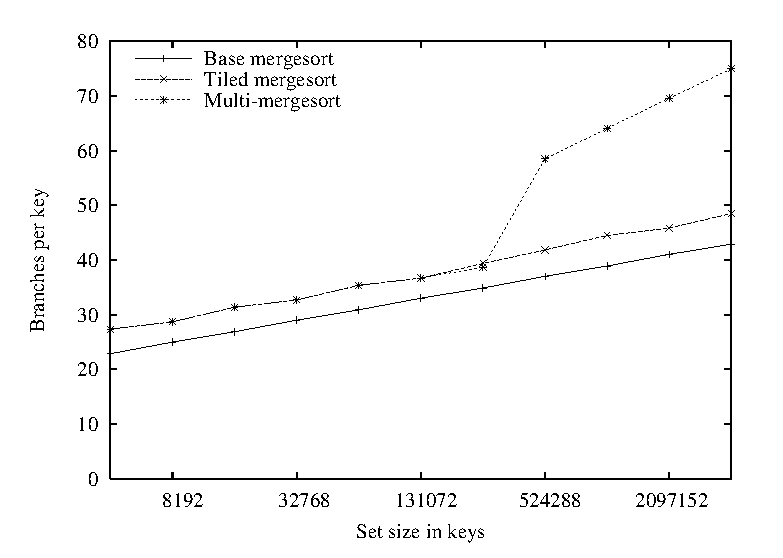
\includegraphics[width=0.48\textwidth]{plots/mergesort_branches_per_key.eps} & 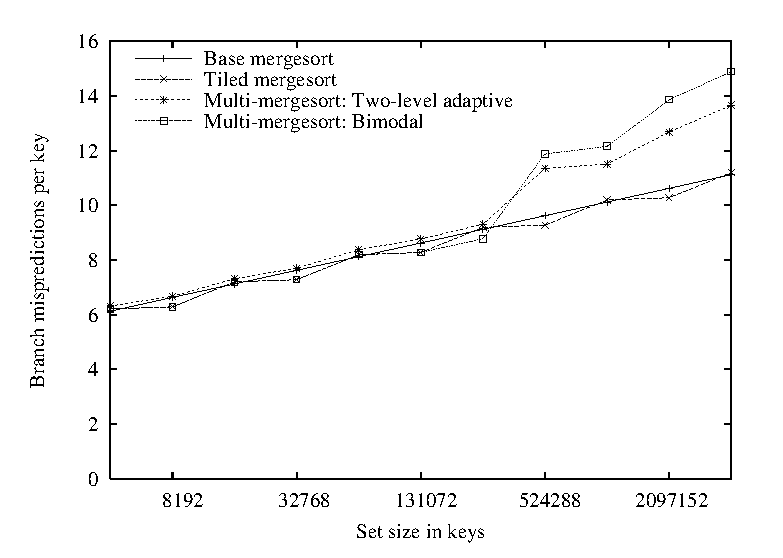
\includegraphics[width=0.48\textwidth]{plots/mergesort_branch_misses.eps} \\
(a) & (b) \\
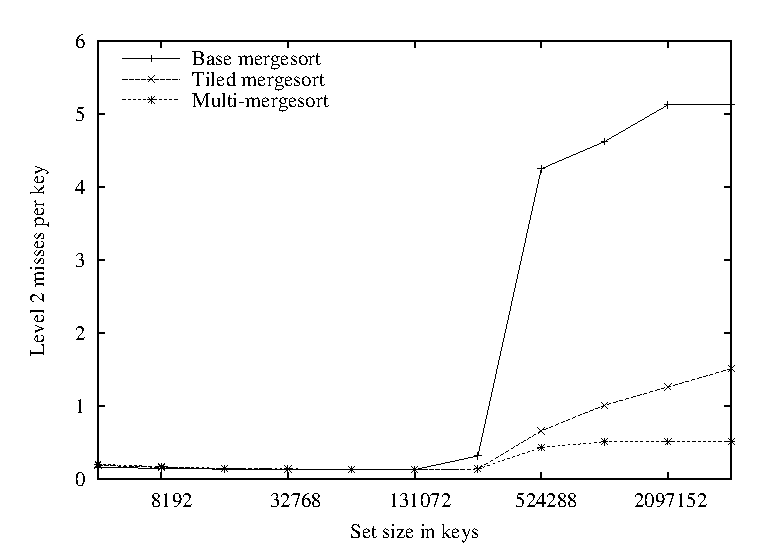
\includegraphics[width=0.48\textwidth]{plots/mergesort_level_2_misses.eps} & 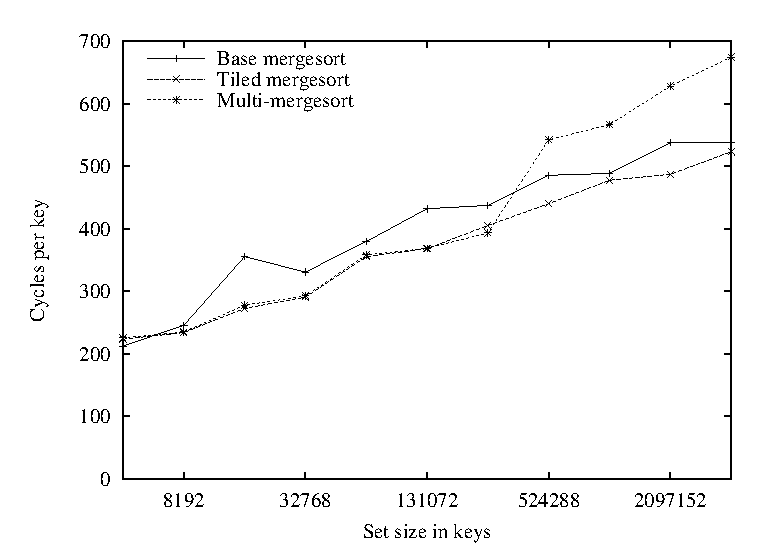
\includegraphics[width=0.48\textwidth]{plots/mergesort_cycle_counts.eps} \\
(c) & (d) \\
\end{tabular}
\caption{(a) Shows the branches per key executed by our mergesort variations.
The sudden increase in the number of executed branches for multi-mergesort
results from the use of the multi-way merge when the data no longer fits within
the cache. (b) Shows the number of mispredictions per key, all predictors had
4096 table entries. Bimodal predictors were used for base and tiled mergesort.
These results were generated using \texttt{sim-bpred}, the two-level adaptive
predictor had a 10-bit history register.  (c) Shows the level 2 cache misses per
key, base mergesort has by far the worst cache behaviour, while multi-mergesort
has slightly better cache performance than tiled mergesort. These results were
generated by using \texttt{sim-cache} to simulate a direct mapped 2MB cache with
32-byte cache lines. Finally (d) shows the cycles per key of our algorithms
measured using Pentium 4 hardware performance counters. Despite
multi-mergesort's superior cache performance, its heightened instruction count
and branch mispredictions mean that the less cache conscious tiled mergesort
performs the best out of the algorithms.}
\label{mergesort_branch_results}
\end{figure}

\section{Quicksort}

Quicksort \cite{Hoare62} is an algorithm which selects a key from its input
called the pivot and then partitions the other keys into two sets, one set
containing keys at most equal to the pivot and another containing keys at least
equal to the pivot. The keys of these sets should appear respectively to the
left and right of pivot in sorted order.  Therefore they can be sorted
independently, each using quicksort.

\subsection{Quicksort Variations}

For our basic quicksort implementation, we make use of a number of improvements
suggested by Sedgewick \citeyear{Sedgewick78}. Firstly, we use an explicit stack
instead of recursing, to save space. Secondly, after partitioning, we always
quicksort the set with the smaller number of elements first.  This reduces the
worst case stack space to $O(\lg n)$ from $O(n)$.  Thirdly, inputs of less than
a certain \texttt{THRESHOLD} (typically \texttt{THRESHOLD} is 10) in size are
not quicksorted at all. Instead, insertion sort is run as a post-pass over the
output of quicksort.  The smallest of the first \texttt{THRESHOLD} keys is used
as a sentinel for insertion sort.  Finally, we use median-of-3 pivoting, greatly
reducing the chances of very unbalanced partitioning and also removing the need
for bounds checks in the inner-loop, thus greatly reducing the instruction
count.

Improvements such as those just described are found in most efficient quicksort
implementations. We also investigated the branch prediction behaviour of cache
conscious quicksort implementations. LaMarca and Ladner \citeyear{LaMarca97}
suggest that instead of running insertion sort as a post-pass over the
quicksorted input, each time quicksort is presented with an input of size less
than \texttt{THRESHOLD} it immediately insertion sorts it. Although this
increases the instruction count, it is more than compensated for by the
resultant drop in cache misses. We refer to this as memory-tuned quicksort.

When quicksort's input fits within a particular level of the cache quicksort has
good cache properties at that level. To combat a dramatic increase in cache
misses when the input does not fit in the cache, LaMarca and Ladner also suggest
multi-quicksort.  Multi-quicksort chooses a set of pivots and performs a
multi-way partition which divides the input into cache sized containers. Each
container is then quicksorted. We leave the precise details of performing a
multi-way partition to elsewhere \cite{LaMarca96a,BiggarGregg05}, it is
sufficient to note that we can decide which container a key should be placed in
by using either a sequential or binary search.

\begin{figure}
\centering
\begin{tabular}{cc}
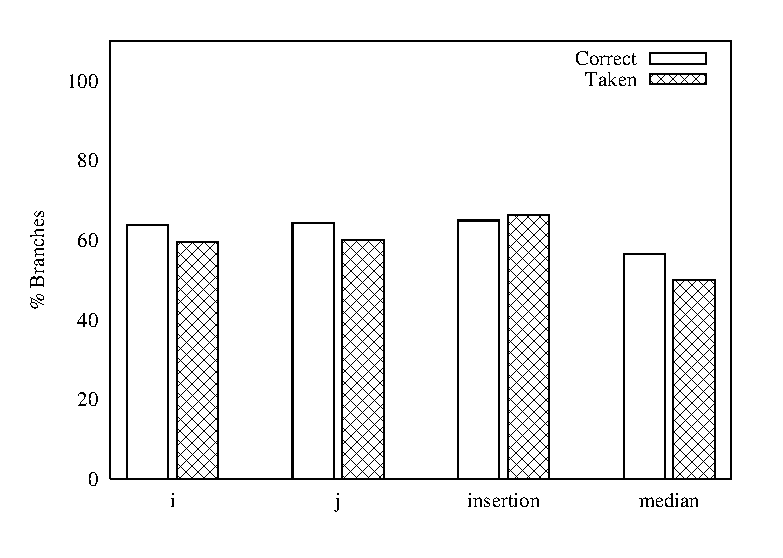
\includegraphics[width=0.48\textwidth]{plots/counter_base_quicksort__median_of_3__0.eps} & 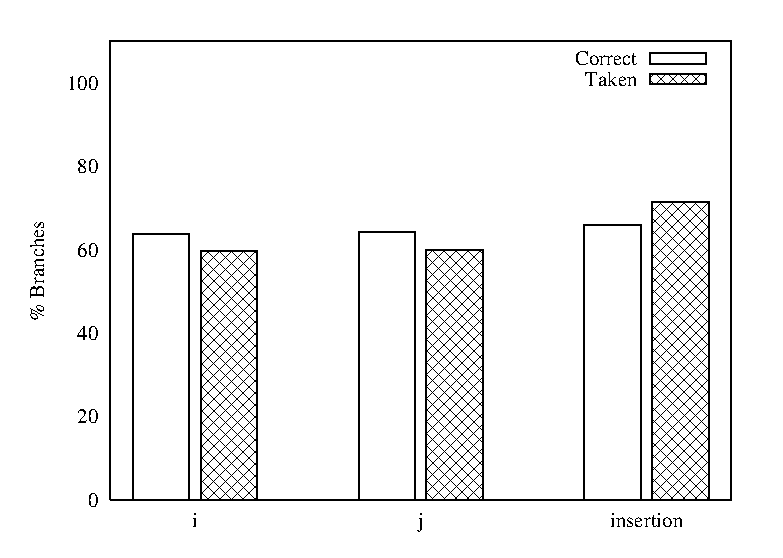
\includegraphics[width=0.48\textwidth]{plots/counter_memory_tuned_quicksort_0.eps} \\
(a) Basic quicksort & (b) Memory-tuned quicksort \\ 
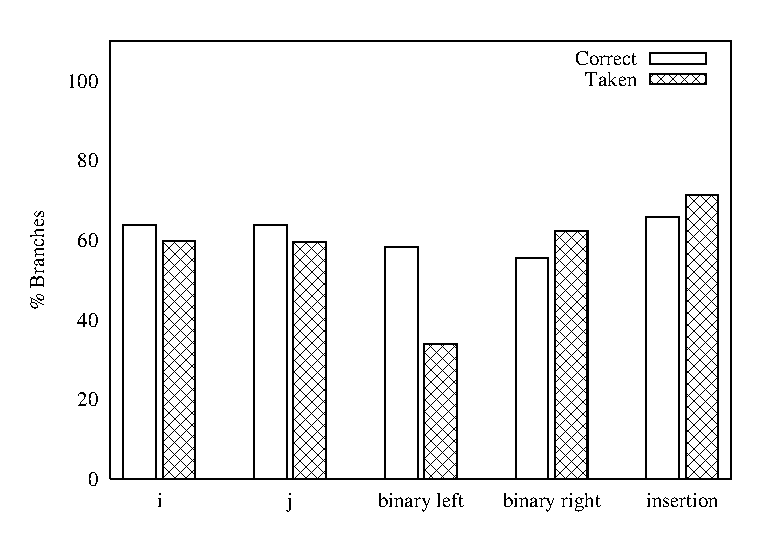
\includegraphics[width=0.48\textwidth]{plots/counter_multi_quicksort__binary_search__0.eps} & 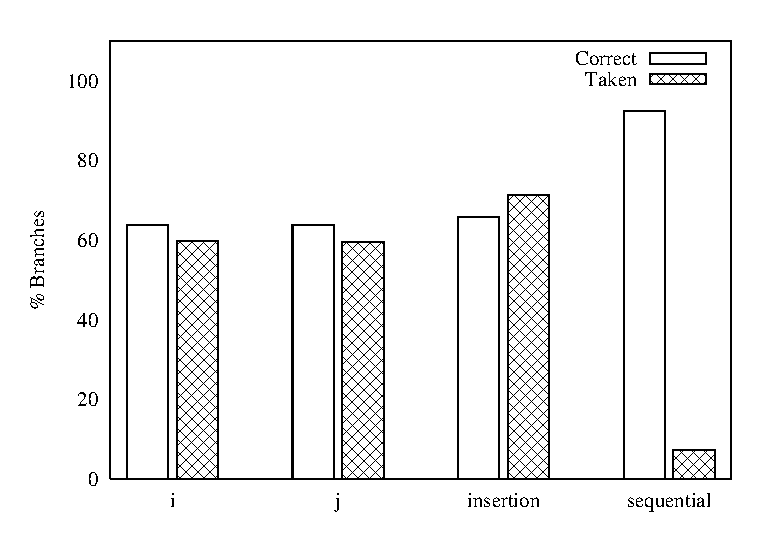
\includegraphics[width=0.48\textwidth]{plots/counter_multi_quicksort__sequential_search__0.eps} \\
(c) Multi-quicksort (binary search) & (d) Multi-quicksort (sequential search)
\end{tabular}
\caption{Overview of branch prediction behaviour in our quicksort
implementations. Every figure shows the behaviour of the $i$ and $j$ branches
when using a median-of-3 pivot. As described in Section
\ref{quicksort_branch_results_text}, these branches are about 60\% biased and
64\% predictable when using the median-of-3. In (a) the \texttt{median} branch
is the combined results of the branches which compute the median-of-3 (these
branches are also executed for (b), (c) and (d)).  Comparing (a) with (b), (c)
and (d), we see that the \texttt{insertion} branch associated with its insertion
sort is slightly less predictable than in the other variations. This is due to
it running as a post-pass. Finally, comparing (c) with (d) we see that the
binary search branches of (c), \texttt{binary left} and \texttt{binary right},
are very unpredictable compared to the \texttt{sequential} branch of (d).  }
\label{branch_prediction_quicksort}
\end{figure}

\begin{figure}
\begin{verbatim}
      pv = a[0];
      i = l, j = r + 1;
      while(true)
      {
              while(a[++i] < pv) ; // i-loop
              while(a[--j] > pv) ; // j-loop
              if(i >= j) break;
              swap(a[i], a[j]);
      }
      swap(a[0], a[j]);
\end{verbatim}
\caption{Quicksort's partition inner-loop. We refer to the inner while loops as
the $i$ and $j$ loops. We refer to their associated branches as the $i$ and $j$
branches respectively.}
\label{partition_code}
\end{figure}

\subsection{Branch Prediction Results}
\label{quicksort_branch_results_text}

Figure \ref{branch_prediction_quicksort} shows the branch prediction results of
our quicksort implementations.  In all figures, the most important branches are
the $i$ and $j$ branches (see Figure \ref{partition_code}), since these are in
quicksort's inner-loop, and are executed more often than any of the other
branches (with the exception of the \texttt{sequential} branch of Figure
\ref{branch_prediction_quicksort}(d)).

The branch prediction behaviour of basic quicksort and memory-tuned quicksort
are similar.  As can be seen in Figure \ref{branch_prediction_quicksort}(b)
quicksort has a slightly lower branch misprediction rate on the
\texttt{insertion} branch. This is because a basic quicksort implementation,
which performs insertion sort as a post-pass, will generate branch
mispredictions on keys chosen as pivots since they never require movement.  In
practice, the over-all reduction in branch misprediction rate from 35\% in basic
quicksort to 34\% in memory-tuned quicksort is probably offset by the branch
misprediction rate of the outer-loop exit in the many insertion sorts executed
by memory-tuned quicksort. However, memory-tuned quicksort has better caching
properties, and so from the point of view of both branch prediction and caching
behaviour this optimization is to be recommended. 

Multi-quicksort results in a 19\% reduction in the number of iterations of the
$i$ and $j$ loops of quicksort's partition inner-loop, though their
misprediction rate remains the same at 37\%. Figure
\ref{branch_prediction_quicksort}(c) shows branch behaviour for multi-quicksort
when using binary search. The binary search branches are highly unpredictable,
being incorrectly predicted 43\% of the time. If multi-quicksort uses sequential
search, the number of executed branches dramatically increases, but these
branches are correctly predicted 92\% of the time, as shown in Figure
\ref{branch_prediction_quicksort}(d). 

The implementations of multi-quicksort have the best cache performance of the
quicksort variations, as Figure \ref{quicksort_plots}(a) shows.  However, the
multi-quicksort implementations also introduce many extra instructions per key
as is seen in Figure \ref{quicksort_plots}(b).  Naturally, the sequentially
searched version introduces more extra instructions than the binary searched
version. However, as described in the previous paragraph, the branches
introduced by binary search are highly unpredictable. As a result,
multi-quicksort using binary search has more branch mispredictions than the
sequential searched version (see Figure \ref{quicksort_plots}(c)), consequently,
despite having identical cache performance, binary searched multi-quicksort
performs worse than the sequentially searched multi-quicksort, as shown in
Figure \ref{quicksort_plots}(d). Of course, on very large data sets (larger than
the $2^{22}$ keys we experimented with), the reduced instruction count of binary
searched multi-quicksort would eventually allow it to out-perform sequentially
searched multi-quicksort.

As Figure \ref{quicksort_plots}(d) shows, our base quicksort implementation
performs the best of all. It seems the improved cache performance of
multi-quicksort is not enough for it to out-perform base quicksort on the data
set sizes we experimented with. Examining the trends of Figure
\ref{quicksort_plots}(a), it seems likely that multi-quicksort would eventually
out-perform base quicksort due to its improved cache performance.  The fact that
base quicksort out-performs memory-tuned quicksort is very difficult to explain.
In the simulations memory-tuned quicksort has the same cache performance and
instruction count, as shown in Figures \ref{quicksort_plots}(a) and
\ref{quicksort_plots}(b). Also in the simulations, memory-tuned quicksort has
slightly fewer branch mispredictions than base quicksort, as Figure
\ref{quicksort_plots}(c) shows. Despite this, base quicksort slightly
out-performs memory-tuned quicksort on our non-simulated hardware test as Figure
\ref{quicksort_plots}(d) shows.

\begin{figure}
\centering
\begin{tabular}{cc}
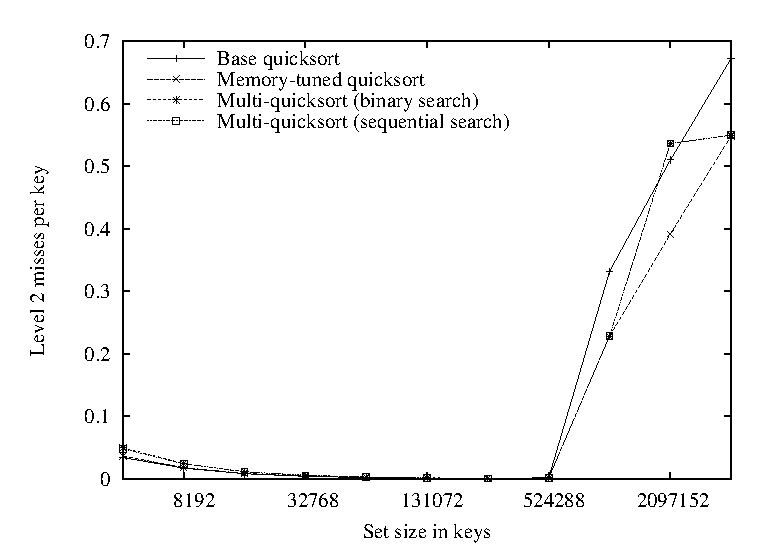
\includegraphics[width=0.48\textwidth]{plots/quicksort_cache_misses.eps} & 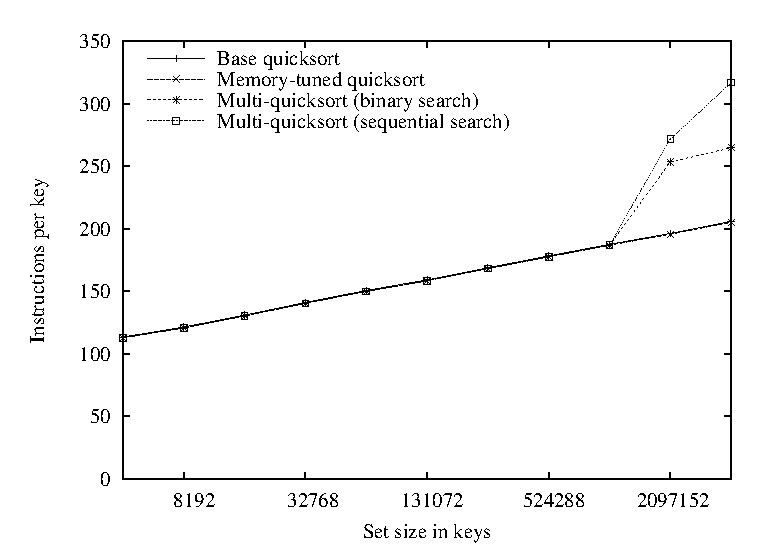
\includegraphics[width=0.48\textwidth]{plots/quicksort_instruction_counts.eps} \\
(a) & (b) \\ 
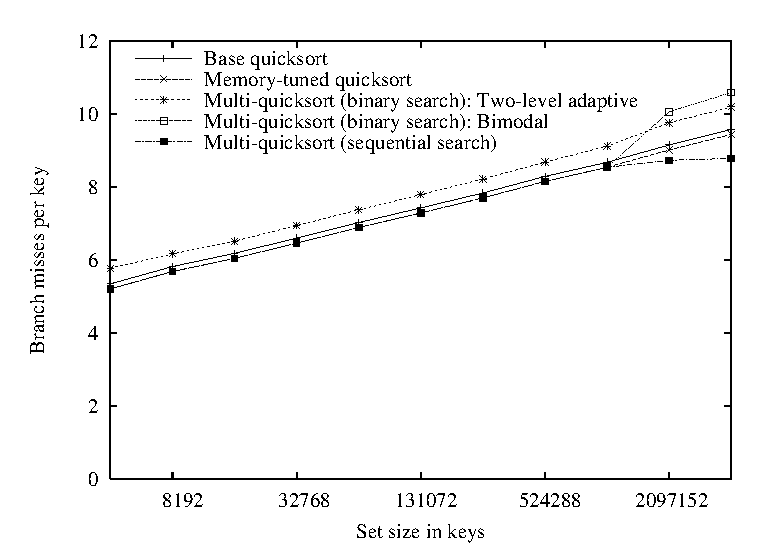
\includegraphics[width=0.48\textwidth]{plots/quicksort_branch_misses.eps} & 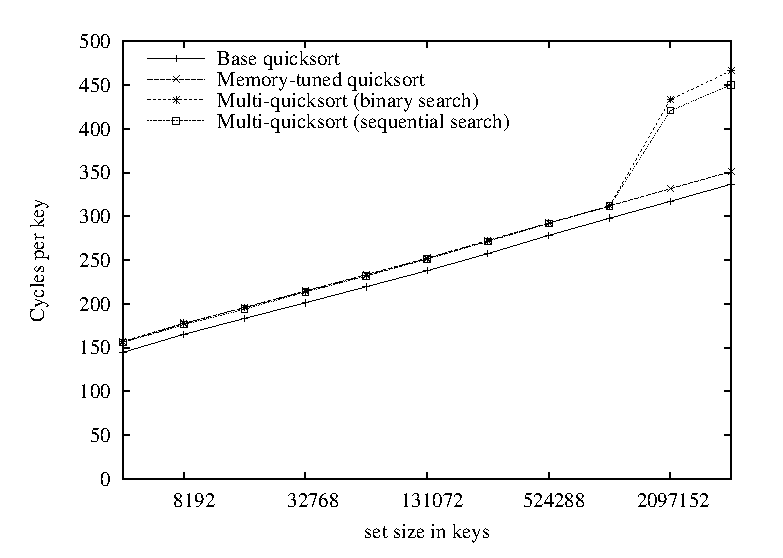
\includegraphics[width=0.48\textwidth]{plots/quicksort_cycles.eps} \\
(c) & (d) \\
\end{tabular}
\caption{(a) Shows the 2nd level cache misses for our quicksort implementations.
As is expected, the multi-quicksort implementations have the best cache
performance. These results were generated using \texttt{sim-cache} to simulate a
2MB direct-mapped cache with 32-byte cache lines.  (b) Shows the instruction
counts of our quicksort implementations, when the data sets no longer fit within
the cache the multi-quicksort implementations show a large increase in
instruction count, these results were also generated using SimpleScalar. (c)
Shows the simulated branch mispredictions per key for our quicksort
implementations. All predictors use 4096 table entries and are bimodal
predictors except where indicated. Multi-quicksort using binary search is the
only implementation which gives varying results from the use of a two-level
adaptive predictor. These results were generated using \texttt{sim-bpred}. (d)
Shows the cycles per key for our quicksort implementations measured using
Pentium 4 hardware performance counters.  }
\label{quicksort_plots}
\end{figure}

\subsection{Pivot Choice}
\label{quicksort_pivot_choice}

The choice of pivot element has a strong influence on the behaviour of the $i$
and $j$ branches (see Figure \ref{partition_code}). Clearly, if the pivot is
chosen as the median of the input then either branch is equally likely to be
taken (i.e. the loop executes) as not taken (i.e.  the loop exits). In this
case, the branches are also on average approximately 50\% predictable.  However,
on average over random input, with a fixed choice of pivot the $i$ and $j$
branches are about 66\% biased (that is, they are taken about 66\% of the time).
It is straightforward to show why this is so. Assume that the data to be
partitioned is a random permutation of $\lbrace 1, \ldots, n \rbrace$.  If the
chosen pivot has rank $q$ then the $i$ branch will be taken with probability $(q
- 1)/n$.  Moreover, the branch will be executed (but not necessarily taken) a
total of $q$ times, since there are exactly $q - 1$ elements to the left of the
pivot. The average bias is given by averaging over all possible choices of pivot
$q$, thus

\begin{equation}
B_{avg}^n = \frac{2}{n(n + 1)}\sum_{q = 1}^n \left(\frac{q - 1}{n} \right) q = \frac{2}{3} - \frac{2}{3n} 
\label{bias_equation}\end{equation}

\noindent
So the bias rapidly approaches 66\% as $n$ increases. With this bias, the $i$
and $j$ branches are about 71\% predictable.  The fact that predictability of
these branches exceeds their biases may at first seem paradoxical. The reason
the branches are more predictable than biased is because the bias is an average.
The average predictability of the $i$ and $j$ branches can be obtained very
simply from Equation \ref{bias_equation} using the steady state predictability
function, $CP$, introduced in Section \ref{bubble_sort}, thus 

\[
P_{avg}^n = \frac{2}{n(n + 1)}\sum_{q = 1}^n CP\left( \frac{q - 1}{n} \right) q
\]

\noindent 
As $n \rightarrow \infty$ we have 
$P_{avg} = \int_0^1 CP(q)\,dq = 3/2 - \pi/4$.  Thus we see $P_{avg}$ is about
0.71. This estimated average predictability is close to what is observed
experimentally when using a fixed pivot over random data, as the predictability
entry of the first row of Table \ref{median_table} shows.

If the pivot is chosen as the median-of-3, then the $i$ and $j$ branches are
about 60\% biased in the taken direction, and about 64\% predictable. It is
especially noteworthy that although median-of-3 gives around a 14\% reduction in
the total number of executed comparison branches, there is actually a 6\%
\textit{increase} in the total number of branch mispredictions. As the pivot
more closely approximates the median of the input, there is a continuing trend
of a reduction in the total number of executed branches, as well as reducing
bias and predictability with an increasing total number of mispredictions, as
Table \ref{median_table} shows.

\begin{table}
\begin{tabular}{|c|c|c|c|c|}
\hline
Median-of & Reduction In $\#$Branches & Bias    & Predictability & Misprediction Increase \\
\hline                                                                                   
1         & 0\%                       & 66.1\%  & 70.6\%         & 0\%                    \\
\hline
3         & 14\%                      & 60.0\%  & 64.3\%         & 6.1\%                  \\
\hline
5         & 16.5\%                    & 57.8\%  & 61.6\%         & 9.2\%                  \\                     
\hline
7         & 17.8\%                    & 56.3\%  & 59.9\%         & 11.8\%                 \\
\hline
9         & 19.6\%                    & 55.1\% & 58.3\%          & 14.3\%                 \\
\hline
\end{tabular}
\caption{The effect of choosing a pivot closer to the median on the prediction
of the $i$ and $j$ branches (the results are the same for both). As a higher
order median is used the bias of the $i$ and $j$ branches is reduced, with a
corresponding reduction in their predictability.  The reductions in the number
of executed branches are relative to a fixed choice of pivot (i.e. median-of-1).
The misprediction increases correspond to the total number of branches
mispredicted with a higher order median compared to a fixed choice of pivot.
These measurements were obtained from our own software simulations of a bimodal
branch predictor. Note that the small number of branches required to compute the
median approximations are included in these results.}
\label{median_table} 
\end{table}

The use of the median-of-3 or higher order median approximation greatly reduces
the chances of the worst case behaviour of quicksort, and on average therefore
results in fewer comparison branches being executed. From an information
theoretic perspective, each comparison branch resolves more uncertainty, or
yields more information, and is hence harder to predict. This observation
applies also to the predictability of the branches used in the binary searched
version of multi-quicksort versus the sequentially searched version. There is a
trade-off to be had between the penalty induced by unpredictable comparisons,
versus the increased instruction count caused by making comparisons more
predictable.

In work concurrent to and independent of our own, Kaligosi and Sanders
\citeyear{Kaligosi+06} have investigated the effect of the choice of pivot on
the performance of quicksort. They found that an artificially skewed pivot gives
better performance than using a random pivot or the median-of-3, due to the
reduction in branch mispredictions. This performance increase is despite the
increased instruction count such an artificially skewed pivot causes; we
describe this work in more detail in Section \ref{RelatedWork}.


\section{Radix Sort}
\label{Radixsort}

The purpose of this paper is to show the relevance of branch mispredictions to
sorting. We now show how to develop a  radix sort \cite{Friend56} implementation
for 32-bit integers that, in all our tests, is more efficient than all other
sorting algorithms presented in this paper.  This is in part due to the tiny
number of branch mispredictions incurred by radix sorting. It is also in part
because radix sort operates in linear worst case time. However, in spite of its
better asymptotic performance a ``step'' for our radix sort is quite costly,
requiring a key to be counted four times and copied four times, with the
counting involving several layers of indirection. In contrast, a step for
quicksort is as simple as a comparison and a possible exchange every few steps. 

The cache performance of radix sort is generally poor compared to algorithms
like mergesort or quicksort. In radix sort, each key is used just once each time
it is in the cache, when the data to be sorted is larger than the cache every
key access will result in a cache miss. On the other hand, mergesort and
quicksort have good temporal locality and use keys repeatedly before they are
ejected from the cache.

\subsection{Memory-tuned Radix Sort}

Our basic radix sort implementation is a typical least significant digit radix
sort. We operate in radix 256, and begin by counting the number of keys with a
particular least significant byte by indexing a table of 256 entries with the
least significant bytes of the keys. The entries of this table are then summed
to store the cumulative count of keys with a smaller least significant byte. Now
each key is placed in an auxiliary array according to the value retrieved by
using its least significant byte to index into the table of cumulative counts.
Before the next iteration, the auxiliary array is written back to the original
array and the sort can proceed on the next most significant byte. We use this
implementation to compare against the simple caching improvements we now
suggest.

We can firstly remove the copying back and forth between the original and
auxiliary array, by just alternating their roles on each step. Since we are
sorting 32 bit integers, the number of iterations is even and the data will end
up sorted in its original location. If the number of steps was odd, an
additional copy would be required at the end. Since radix sort is out-of-place,
we might consider aligning its two arrays as we did with mergesort (see Section
\ref{mergesort_variations}). However, radix sort does not access its arrays in
the same regular fashion that mergesort does and so is unlikely to benefit from
such a change. Indeed, we implemented a double-aligned radix sort and did not
observe any performance gains.  Finally, we use an improvement suggested by
LaMarca and Ladner \citeyear{LaMarca97}, where the counting of the next most
significant bytes is begun during their preceding iteration. We refer to this
optimized version of radix sort as memory-tuned radix sort.

In our basic radix sort implementation, the first array is accessed 3 times and
the second array twice, in each of the four iterations over the four bytes in
the 32-bit integers. This gives 20 accesses in total.  In memory-tuned radix
sort each key of the two arrays is accessed only nine times in total.  At the
start, it traverses the original array once to count the least significant
bytes. It then iterates four times, positioning the keys based on the previously
established counts. These four iterations cause a total of eight accesses,
because each array is accessed once per iteration.

\subsection{Results}

\begin{figure}
\centering
\begin{tabular}{cc}
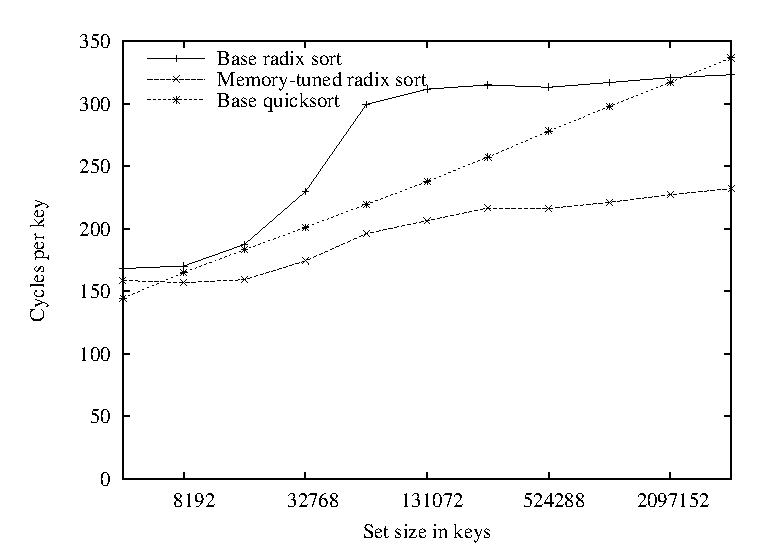
\includegraphics[width=0.48\textwidth]{plots/radix_cycles.eps} & 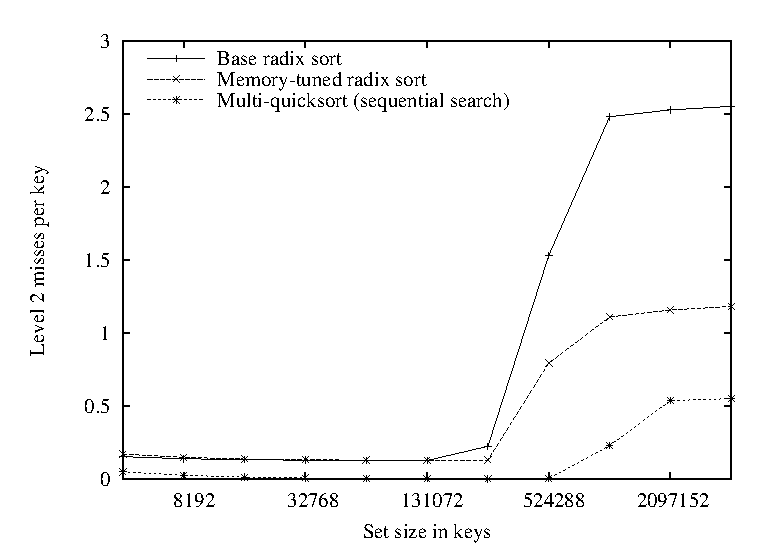
\includegraphics[width=0.48\textwidth]{plots/radix_versus_quick_level_2_misses.eps} \\
(a) & (b) \\
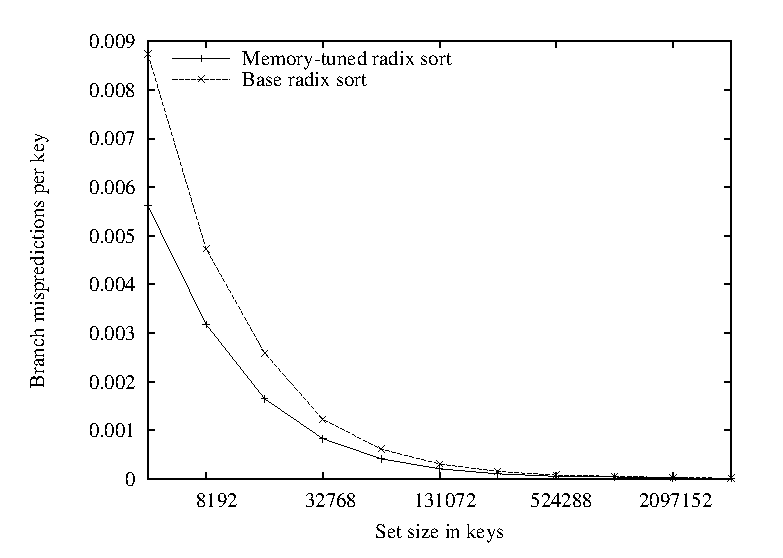
\includegraphics[width=0.48\textwidth]{plots/radix_branch_misses.eps} & 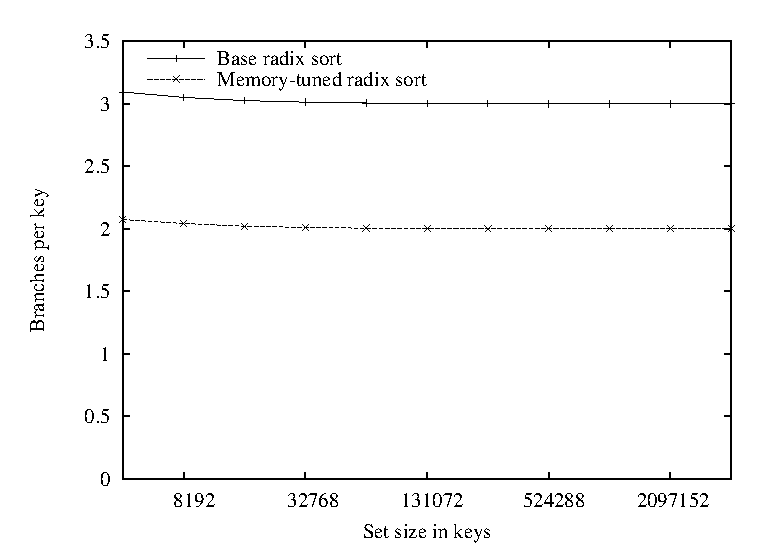
\includegraphics[width=0.48\textwidth]{plots/radix_branches.eps} \\
(c) & (d) \\
\end{tabular}
\caption{(a) Shows the cycles per key of our radix sort implementations
alongside our base quicksort implementation, measured using Pentium 4 hardware
performance counters. (b) Shows the level 2 cache misses incurred by our radix
sort implementations and a multi-quicksort implementation for a 2MB direct
mapped cache with 32-byte cache lines. These results were generated using
\texttt{sim-cache}.  (c) Shows the average branch mispredictions per key
incurred by our radix sort implementations while using bimodal predictors with
4096 table entries, the results for two-level adaptive predictors are extremely
similar. Finally, (d) shows the average number of branches per key executed by
our  implementations. The results of (c) and (d) were generated using
\texttt{sim-bpred}.}
\label{radixsort_results_pictures}
\end{figure}

Our radix sort implementation requires fewer processor cycles per key than even
our base quicksort implementation as Figure \ref{radixsort_results_pictures}(a)
shows. 

Figure \ref{radixsort_results_pictures}(b) shows the level 2 cache misses for
our basic and memory-tuned implementations.  The number of level 2 cache misses
is only slightly higher than we measured for quicksort while the array fits
inside the cache, presumably because radix sort is out-of-place.  We note that
when the array no longer fits inside the cache the memory-tuned implementation
has approximately half the number of misses per key (1.25) than the basic
version (2.5). When the data no longer fits inside the cache there should be
about one miss for each key per pass per cache line.  Each cache line can fit 8
keys, and thus we expect the observed 2.5 misses per key since there are 20
passes in total.  likely exceeds this because of the irregular fashion of the
array indexing in each pass. Similary, in memory-tuned radix sort we expect
slightly below 1.25 misses per key since there are 9 passes in total.

The large advantage of radix sort is its almost complete lack of branch
mispredictions however. Figure \ref{radixsort_results_pictures}(c) shows the
tiny number of branch mispredictions incurred by radix sort. It also executes a
similarly tiny number of branch instructions as Figure
\ref{radixsort_results_pictures}(d) shows. 

\section{Related work} 
\label{RelatedWork}
% The IBM 7030 "Stretch" supercomputer was the first general-purpose
% pipelined architecture \cite{Bloch59}. Released in 1959 it had a
% four-stage pipeline and many other architectural innovations that are
% now commonplace in desktop and even embedded computers. 

We present the first large-scale systematic study of branch prediction and
sorting. However, researchers have been aware for many years that the branches
in comparison-based sorts cause problems on pipelined architectures. As early as
1972 Knuth commented on the ``ever-increasing number of `pipeline' or `number
crunching' computers that have appeared in recent years'' whose ``efficiency
deteriorates noticeably in the presence of conditional branch instructions
unless the branch almost always goes the same way''. He also notes that ``radix
sorting is usually more efficient than any other known method for internal
sorting on such machines'' (the same comment appears in \cite{KnuthVol3_98}).
Most likely, Knuth was referring to the IBM 7030 ``Stretch'' computer (released
in 1961 with a four-stage pipeline), Seymour Cray's Freon-cooled CDC 6600
supercomputer (released 1964), or other early supercomputers which used
pipelining in the execution of general-purpose instructions.

A number of other authors have considered optimized implementations of sorting
algorithms for more recent single-processor machines. Nyberg \textit{et al}
\citeyear{Nyberg+94} present a quicksort-based algorithm for RISC architectures.
They found that the main limit on performance was cache behaviour, and did not
mention branch prediction even once. Bentley and McIlroy \citeyear{Bentley+93}
implemented a highly-tuned quicksort, to be used in the \texttt{qsort} function
of the standard C library. Again, they did not consider branch prediction,
perhaps because the first desktop processors with dynamic branch predictors
(such as the DEC Alpha 21064, MIPS R8000 and Intel Pentium) were only just
appearing around that time.

Agarwal \citeyear{Agarwal96} developed an optimized algorithm for sorting random
records on an IBM RS/6000 RISC machine. His is the first published algorithm
that we are aware of that deliberately attempts to improve performance by
eliminating branch mispredictions. First, it uses the seven higher order bits of
the key to divide the data into 128 buckets. Each of these buckets is
radix-sorted. However, before the radix sort is reaches the lowest order bits,
the probability of any adjacent pair of keys being out of order is extremely
low, because the problem states that the data is guaranteed to be random. In the
final stage, the algorithm checks that large runs of keys are correctly ordered
using subtraction and bitwise operations, and only sorts a section if some key
is found to be out of order. Although Agarwal's techniques are interesting, they
are very dependent on the randomness of the data; it is easy to construct
commmon cases that would result in very poor performance. Nonetheless, the work
is interesting because it shows the effectiveness of radix sorting techniques on
pipelined architectures.

A recent trend in optimizing algorithms for FFT, linear algebra, and digital
signal processing has been to automatically generate and evaluate very large
numbers of variants of the algorithm.  A similar approch is used by Li
\textit{et al} \citeyear{Li+05} to automatically generate sorting algorithms
that are tuned to the architecture of the target machine and the characteristics
of the input data. They identify six sorting primitives, which can be combined
to construct a sorting algorithm.  A large number of combinations are tested,
using a genetic algorithms search to find the most efficient. The resulting
implementations are, in many cases, significantly faster than commercial sorting
libraries.  Although they do not consider branch prediction explicitly, they
find that the implementations that perform best usually use radix sort for a
large part of the sorting process.

Sanders and Winkel \citeyear{Sanders+04} investigate the use of
\emph{predicated} instructions on Intel Itanium 2 processors. In addition to its
normal inputs, a predicated instruction takes a predicate register input. If the
value in the predicate register is true, the instruction takes effect; otherwise
it does not. Predication is normally implemented by the instruction being
executed regardless of whether the predicate is true. However, its result is
only \textit{written back} to a register or memory if the predicate is true.
Although predicated instructions use execution resources regardless of whether
they are allowed to write back, they allow conditional branches to be
eliminated.  Sanders and Winkel show how the partition step in quicksort can be
rewritten to use predicated instructions on an Itanium 2, a highly
instruction-level parallel machine. Itanium 2 provides large numbers of parallel
functional units and registers which make such trade-offs worthwhile. 

\comment{ In preliminary experiments, we found that Sanders and Winkel's work is
difficult to reproduce on a Pentium 4 based machine. The only predicated
instruction supported on the Pentium 4 is the conditional move instruction. We
found that rewriting quicksort's loops so that they are suitable for predication
reduces their efficiency and also increases the number of simultaneously live
variables.  Since the Pentium 4 has only eight general purpose registers the
number of simultaneously live variables exceeded the number of available
registers, reducing efficiency. In addition, we also discovered that on the
Pentium 4 conditional moves are surprisingly expensive.  } Mudge \textit{et al}
\citeyear{Mudge+96} examine the behaviour of the $i$ and $j$ comparison branches
in randomized quicksort, as an example to demonstrate a general method for
estimating the limit on the predictability of branches in a program. They argue
that the optimal predictor for these branches would keep a running count of the
total number of array elements examined so far that are greater than the pivot.
If the majority of the elements examined so far are greater than the pivot, the
next element is predicted as greater than the pivot, and vice versa. They
estimate that this approach will give a prediction accuracy of 75\%, which is
close to our result for these branches, using a bimodal predictor.  This shows
that a bimodal predictor is close to optimal for randomized quicksort's
branches, since $P_{avg}$ of Section \ref{quicksort_branch_results_text} is
about 0.71.

Brodal \textit{et al} \citeyear{Brodal+05} examine the adaptiveness of
quicksort.  They find that although randomized quicksort is not adaptive (i.e.
its asymptotic analysis does not improve with respect to some measure of
presortedness), its performance is better on data with a low number of
inversions. They justify this by showing that the expected number of element
swaps performed by randomized quicksort falls as the number of inversions does.
The number of branch mispredictions is roughly twice the number of element
swaps, because two branch mispredictions tend to occur when the two while loops
of the partition code exit (see Figure \ref{partition_code}).  Furthermore they
note that the branch mispredictions are the dominant part of the running time of
randomized quicksort. This provides an empirical relation between the
presortedness of the input, randomized quicksort's performance, and the number
of branch mispredictions. 

In closely related work Brodal and Moruz \citeyear{BrodalMoruz05} provide a
lower bound on the number of branch mispredictions a comparison-based sorting
algorithm must incur based on the number of comparisons it performs. They also
show that a mergesort variation can achieve this lower bound based on the number
of comparisons it performs, although they do not provide experimental
performance characteristics. They also extend their results to adaptive sorting
algorithms

In recent work conducted independently of our own, Kaligosi and Sanders
\citeyear{Kaligosi+06} investigate the choice of pivot on the performance of
quicksort. They examine $\alpha$-skewed pivoting, that is, where the pivot has
rank $\alpha n$ when sorting $n$ keys. They examine the performance of quicksort
when the pivot is determined randomly, from the median-of-3, or is the true
median (i.e. a 1/2-skewed pivot). They show that using a 1/10-skewed pivot gives
a performance increase over all the aforementioned pivot choices. This is
despite the increase in instruction count that a deliberately skewed pivot
causes.

\section{Conclusion}

This paper has presented the first large scale study on the characteristics of
branch instructions in all of the most common sorting algorithms. We noted that
except where the sorting algorithms involve reasonably complicated flow control
(i.e. shellsort, multi-mergesort, multi-quicksort), bimodal predictors preform
just as well as two-level adaptive predictors. Indeed we noted that for shaker
sort a bimodal predictor out-performs a two-level adaptive predictor.

Of the elementary sorting algorithms we noted that insertion sort, causing just
a single misprediction per key, has the best branch prediction characteristics.
On the other hand, bubble and shaker sort operate in a manner which causes
surprisingly unpredictable branches.

Sorting (and indeed, searching) algorithms have been designed to minimize the
number of comparisons necessary in the worst case. However, minimizing the
number of comparisons makes each comparison less predictable. When a branch is
mispredicted, there is often a large penalty on modern processors.  There is
therefore a tension between reducing the number of executed comparisons and the
penalty associated with increasing the chance of branch mispredictions. This
tension is especially evident in the choice of pivot for quicksort.

Since cache optimizations are now recognized as very important, we have also
noted the affect that these cache optimizations have on the branch prediction
behaviour of sorting algorithms. In particular we provided performance results
for cache optimized versions of quicksort, mergesort, heapsort and radix sort.

Our study provides concrete results of the branch prediction characteristics for
a large number of sorting algorithms, accompanied with the relevant analysis.
These branch prediction results have been obtained for realistic dynamic
predictors, using a variety of configurations of bimodal and two-level adaptive
predictors. 

\appendix

\section{Appendix: Steady State Predictability}
\label{appendix_SSP}

In Sections \ref{bubble_sort}, \ref{heapsort_branch_results_text} and
\ref{quicksort_branch_results_text} we made use of the steady state
predictability function $CP$. When a branch instruction is executed repeatedly
with a known probability $p$ of being taken, $CP(p)$ gives a good estimate of
the probability that it will be correctly predicted.

The bimodal predictor associated with a branch instruction can be thought of as
a Markov chain. Note that we are thus assuming that successive branches are
independent. If the branch has probability $p$ of being taken then the
transition matrix of the associated Markov chain is

\[
M = 
\left[
\begin{array}{llll}
p   & p   & 0   & 0 \\
1-p & 0   & p   & 0 \\
0   & 1-p & 0   & p \\
0   & 0   & 1-p & 1-p \\
\end{array}
\right]
\] 

\noindent
The steady state probabilities are given by $s$ such that $Ms = s$.
Since the steady state probabilities sum to one this can be reduced to solving
a $3 \times 3$ linear system. The resultant probabilities are given by

\[
\left[ 
\begin{array}{c}
P(ST) \\
P(T) \\
P(NT) \\
P(SNT) \\
\end{array}
\right]
=
\frac{1}{2p^2 - 2p + 1}
\left[
\begin{array}{c}
p^3 \\
p^2(1 - p) \\
p(1 - p)^2 \\
(1 - p)^3 \\
\end{array}
\right]
\]

\noindent 
Here $P(ST)$, $P(T)$, $P(NT)$ and $P(SNT)$ denote the respective
probabilities of the predictor states strongly taken, taken, not-taken and
strongly not-taken described in Section \ref{branch_prediction}. A branch is
correctly predicted with probability $p$ if we are in the strongly taken or
taken state. Similarly, a branch is correctly predicted with probability $1 - p$
if we are in the strongly not-taken or not-taken state. Thus,

\[
CP(p) = p\left[P(ST) + P(T)\right] + (1 - p)\left[P(SNT) + P(NT)\right]
\]

\noindent
This equation simplifies to Equation \ref{CP_equation} of Section \ref{bubble_sort}.
\bibliographystyle{acmtrans}
\bibliography{paper}
\begin{received}
\end{received}
\end{document}
